%% ****** Start of file aiptemplate.tex ****** %
%%
%%   This file is part of the files in the distribution of AIP substyles for REVTeX4.
%%   Version 4.1 of 9 October 2009.
%%
%
% This is a template for producing documents for use with 
% the REVTEX 4.1 document class and the AIP substyles.
% 
% Copy this file to another name and then work on that file.
% That way, you always have this original template file to use.


\documentclass[aip,graphicx]{revtex4-1}
%\documentclass[aip,reprint]{revtex4-1}

\usepackage{graphicx}
\usepackage[caption=false]{subfig}
\usepackage{array}
\usepackage{amsmath}
\usepackage{bm}
\usepackage{auto-pst-pdf}
\usepackage{psfrag}
\usepackage{pstricks}

\newcommand{\sym}[1]{\text{#1}}
\newcommand{\dif}{\mathrm{d}}
\newcommand{\degree}[1]{#1 \: ^{\circ}}
\newcommand{\degC}[1]{#1 \; ^{\circ} \text{C}}
\newcommand{\degCpm}[2]{#1 \pm #2 \; ^{\circ} \text{C}}
\newcommand{\pder}[2][]{\frac{\partial#1}{\partial#2}}
\newcommand{\der}[2][]{\frac{\text{d}#1}{\text{d}#2}}
\newcommand{\matder}[2][]{\frac{\text{D}#1}{\text{D}#2}}
\newcommand{\secondder}[2][]{\frac{\text{d}^2#1}{\text{d}#2}}
\newcommand{\vect}[1]{\bm{#1}}

\draft % marks overfull lines with a black rule on the right

\begin{document}

% Use the \preprint command to place your local institutional report number 
% on the title page in preprint mode.
% Multiple \preprint commands are allowed.
%\preprint{}

%\title{Influence of the film thickness on the spreading regimes of a viscous drop spreading on an identical film} %Title of paper
\title{Sinking, wedging, spreading -- viscous spreading on an identical layer}

% repeat the \author .. \affiliation  etc. as needed
% \email, \thanks, \homepage, \altaffiliation all apply to the current author.
% Explanatory text should go in the []'s, 
% actual e-mail address or url should go in the {}'s for \email and \homepage.
% Please use the appropriate macro for the type of information

% \affiliation command applies to all authors since the last \affiliation command. 
% The \affiliation command should follow the other information.

\author{Nico Bergemann}
\author{Matthias Heil}
\author{Anne Juel}
%\email[]{Your e-mail address}
%\homepage[]{Your web page}
%\thanks{}
%\altaffiliation{}
\affiliation{The University of Manchester}

% Collaboration name, if desired (requires use of superscriptaddress option in \documentclass). 
% \noaffiliation is required (may also be used with the \author command).
%\collaboration{}
%\noaffiliation

\date{\today}

\begin{abstract}
% insert abstract here
 We investigated experimentally and computationally the viscous spreading of a sessile drop on an identical layer.
 A practical application of this process is spray coating during which subsequent drops spread on an existing layer of the same fluid.
 We performed spreading experiments on a uniform layer as well as on a dry substrate and characterised the driving forces in both cases.
 In the case of spreading on a layer the flow is governed by viscous forces, whereas the spreading on a dry substrate is governed by surface tension.
 We then performed computational simulations of the drop spreading on an identical layer using the finite element method (FEM), as implemented in \texttt{oomph-lib}.
 These computations showed excellent agreement with the experiments.
 Through further computations we established distinct spreading regimes depending on the thickness of the layer.
 For very thick fluid layers the drop primarily sinks into the layer instead of spreading radially.
 On the other hand, for very thin layers the drop spreads similarly to a drop on dry substrate, where the spreading is governed by gravity.
 For intermediate layer thicknesses the drop spreads through an advancing wedge which is sustained by fluid flow from the drop into the layer.
\end{abstract}

\pacs{}% insert suggested PACS numbers in braces on next line

\maketitle %\maketitle must follow title, authors, abstract and \pacs

% Body of paper goes here. Use proper sectioning commands. 
% References should be done using the \cite, \ref, and \label commands
\section{Introduction}
\label{sec:introduction}
%\subsection{}
%\subsubsection{}

The spreading of liquids on solid substrates has received a lot of attention among the research community \cite{de1985wetting, bonn2009wetting}.
Another area of interest is the spreading of a liquid on top of another (immiscible) liquid \cite{fraaije1989dynamics, joos1977spreading}.
While these two configurations of droplet spreading are well investigated, limited research has been performed in the spreading of a sessile Newtonian drop on a layer of the same fluid \cite{tanner1979spreading, cormier2012beyond, chebbi1999capillary}.
Here we investigate the spreading of a Newtonian glucose syrup on a thick layer of the same fluid and find that in this case the flow is governed by a competition of viscous and gravitational forces.
Moreover, we show that for the spreading on a solid substrate the well established spreading law of $R \propto t^{1/10}$ is obtained, which describes flow which is governed by a competition of surface tension and gravity \cite{bonn2009wetting}.

\section{Experiments}
\label{sec:experiments}

\subsection{Experimental setup}

\subsubsection{Experimental apparatus}

\begin{figure}[!h]
\centering
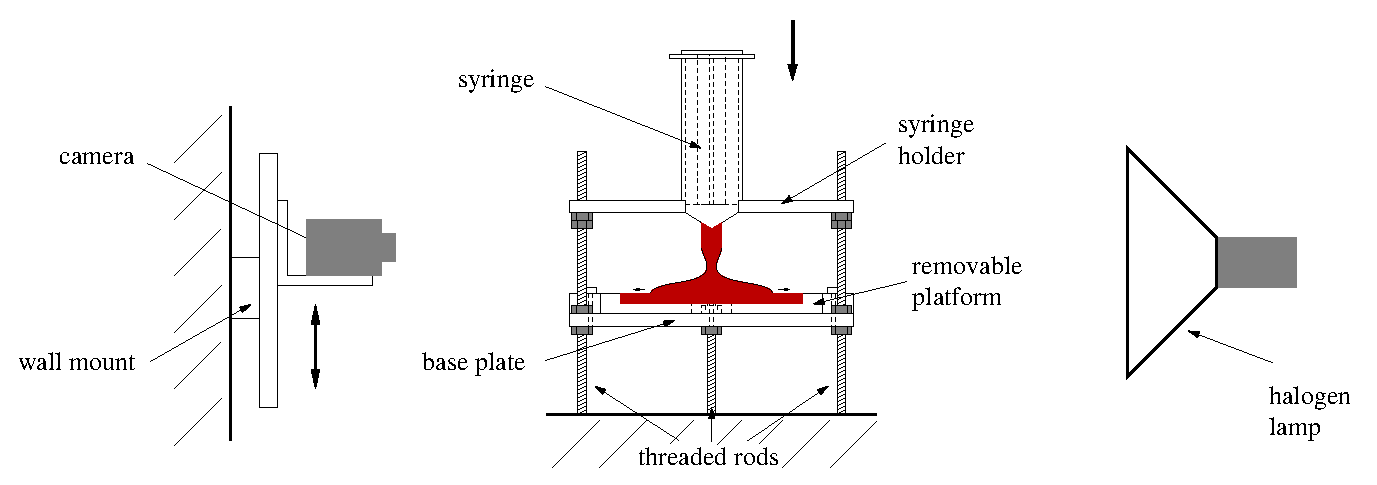
\includegraphics[width=0.99\textwidth]{figures/experimental_apparatus.eps}
\caption{Schematic side-view diagram of the experimental apparatus.}
\label{fig:experimental_apparatus}
\end{figure}

A schematic diagram of the side-view of the experimental apparatus is shown in figure \ref{fig:experimental_apparatus}.
The working part of the setup is a perspex base plate placed on three rigidly mounted threaded poles.
The perspex plate is secured and levelled using nuts.
Levelling is crucial, because otherwise non-axisymmetric instead of the desired axisymmetric spreading is promoted. 
The base plate features three threaded holes, which are used to secure a removable platform with nylon screws.
The top surface of the removable platform features a circular trough with a diameter of 60.5 mm and depth of 2 mm in order to create a layer of fluid.
For the spreading experiments we deposited the fluid using a standard 10 ml plastic screwhead syringe with a nozzle of an outer diameter of 9.22 mm. 
Because of the high viscosity of the glucose syrup we drilled out and smoothed its outlet to create an outlet diameter of 8 mm. 
In order to ensure controlled deposition of fluid, we placed the syringe in a removable holder as shown in figure \ref{fig:experimental_apparatus}. 
The holder consists of a perspex tube which fitted snugly into a central hole in the plate and was bonded into position with perspex cement. 
The syringe holder rests on nuts as shown in figure \ref{fig:experimental_apparatus}, which are also used to level the holder. 
As in the case of the perspex base plate, levelling is crucial, as otherwise non-axisymmetric deposition may result.
A camera (Pulnix TM-6740CL), adjustably mounted on the wall, captures side-view images of the drop which is backlit with a halogen lamp.
The maximum frame rate of the camera is 200 frames per second and the resolution of the grey-scale images is 640x480 pixels.

%\subsubsection{Experimental procedure}

\subsubsection{Sample preparation}

Glucose syrup is a transparent, highly viscous Newtonian liquid.
For the experiments we filled approximately 400 ml of the syrup into a standard low-form 600 ml glass beaker. 
In order to enhance the contrast in the images, we dyed the syrup using red and green food colouring. 
Mixing of the dye entrained air bubbles, which were left to rise out of the fluid overnight.

\subsubsection{Measurement of the material properties}

We measured the density of the glucose syrup at the laboratory temperature of $\degCpm{20.3}{0.2}$, using a standard 50 ml low-form glass beaker. 
First, we determined the weight of the empty beaker using a balance (OHAUS PRECISION Standard) with an accuracy of $\pm 0.001$ g. 
Then we filled the 40 ml beaker from the mixture in the 600 ml beaker using the syringe with the enlarged nozzle. 
We filled the beaker up to 50 ml in increments of 10 ml. 
After each increment we determined the mass of the beaker with syrup. 
For each of these five measurements we calculated the density as $\rho=m_{\sym{glucose}}/V_{\sym{glucose}}$, where $m_{\sym{glucose}}$ is the mass of glucose syrup and $V_{\sym{glucose}}$ its volume.

{\renewcommand{\arraystretch}{1.2}
 \begin{table}[!ht]
 \begin{center}
 \begin{tabular}{c | c | c | c}
  $V_{\sym{glucose}}$ in ml & $m_{\sym{tot}}$ in g & $m_{\sym{glucose}}$ in g & $\rho$ in kg/m$^3$ \\ 
   \hline
   0 & 38.680 & 0.0 &  \\
   10 & 52.456 & 13.776 & 1377.6 \\
   20 & 66.201 & 27.521 & 1376.1 \\
   30 & 79.976 & 41.296 & 1376.5\\
   40 & 93.316 & 54.636 & 1365.9 \\
   50 & 107.066 & 68.386 & 1367.7
 \end{tabular}
 \caption{Density measurements for glucose syrup.}
 \label{tab:glucose_density}
 \end{center}
 \end{table}}

The results are shown in table \ref{tab:glucose_density}, where the mass of the empty beaker ($V_{\sym{glucose}}=0$ ml) is given as 38.68 g. 
For a more accurate result we averaged the density across these measurements, giving in a mean density of $1372.8 \; \pm \; 4.9 \; \sym{kg}/\sym{m}^3$.

The viscosity of syrup depends exponentially on temperature \cite{llewellin2002rheology} and we therefore measured it at 20.0, 20.1, 20.3, 20.5 and $\degC{21.0}$ using a Brookfield R/S-Plus (SST) rheometer with a concentric cylinder CC25 geometry and temperature control. 
We performed shear rate measurements with linear increase from zero to a maximum value of $25 \; \sym{s}^{-1}$ with increments of $1 \; \sym{s}^{-1}$, applying a cycle of shear rate increase and immediate decrease. 
The total experiment time was 50 s, with one measurement taken per second.
Hence, for each temperature we recorded 50 viscosity measurements and these experiments confirmed that the viscosity of glucose syrup is independent of the shear rate and hence behaves as a Newtonian fluid in the investigated range.

{\renewcommand{\arraystretch}{1.2}
 \begin{table}[!ht]
 \begin{center}
 \begin{tabular}{c | c}
  Temperature in $\degC{}$ & Viscosity $\mu$ in Pa.s \\ 
   \hline
   20.0 & $43.62 \; \pm \; 0.22$ \\
   20.1 & $43.72 \; \pm \; 0.19$ \\
   20.3 & $43.61 \; \pm \; 0.23$ \\
   20.5 & $42.51 \; \pm \; 0.21$ \\
   21.0 & $40.34 \; \pm \; 0.19$\\
 \end{tabular}
 \caption{Viscosity measurements for glucose syrup at different temperatures.}
 \label{tab:glucose_viscosity}
 \end{center}
 \end{table}}
 
The averaged values for the dynamic viscosity $\mu$ are presented in table \ref{tab:glucose_viscosity}. 
The viscosities at $20.0 - \degC{20.3}$ are similar and not significantly different. 
However, at temperatures of 20.5 and $\degC{21.0}$, the viscosity is decreased.

We did not explicitly determine the surface tension of glucose syrup, but use the literature \cite{montanez2013influence} value of 55.0 $\pm 0.6$ N/m.

\subsubsection{Deposition of a sessile drop}

For each spreading experiment we recorded the ambient temperature of the laboratory. 
Before the actual experiments, the images were calibrated against an object of known size.
We performed the spreading experiments on both a dry perspex substrate and a layer of glucose syrup.
In case of spreading on a layer, we took out the removable platform and filled it with the dyed glucose syrup. 
In order to create a uniform layer in the trough, we scraped across the platform with a straight-edged plastic piece. 
This scraping resulted in a layer which was thinner than the 2 mm depth of the trough, which is explained in more detail in section \ref{sec:creating_layer} below.
After filling, we placed the platform on the observation assembly and secured it with the nylon screws. 
Next, we partially filled the syringe from the beaker and emptied it again in order to remove the air entrapped in the syringe nozzle and to replace it with syrup instead. 
Then we filled the syringe with 5 ml of glucose syrup and cleaned the outside of the nozzle with a dry paper towel.
We placed the filled syringe in the perspex tube of the syringe holder and placed the holder onto the threaded poles of the observation platform such that it rested on all three nuts, as shown in figure \ref{fig:experimental_apparatus}. 
We reduced the frame rate of the camera to 20 frames per second, by setting the skip count (the number of frames to be skipped) to 9 for the image sequence acquisition within NI Vision Assistant. 
Once we started the image acquisition, we pushed down the plunger of the syringe manually and recorded the spreading. 
After the image acquisition had finished, we saved the images, and removed the syringe holder and removable platform. 
We cleaned the platform, plastic scraper and syringe under hot, running water and thoroughly dried them with paper towels.

\subsubsection{Creating a uniform layer}
\label{sec:creating_layer}

For the spreading experiments on a layer of fluid the challenge was to create a uniform layer.
However, for glucose syrup this is not straightforward, because of its high viscosity.
Filling the through with the exact amount of fluid to create a layer of known depth and allowing it to settle intuitively seems the best approach.
But for such a high viscosity fluid the settling into a uniform layer would take an infinite amount of time.
In addition, the glucose syrup crystalises at the surface, if it is exposed to air for a long time and the observed behaviour would no longer be that of a drop spreading on an identical layer.
For these reasons our approach to create a uniform layer was to fill the trough with an excess amount of syrup and then scraping across the trough to create an even layer.
 
\begin{figure}[!ht]
\centering
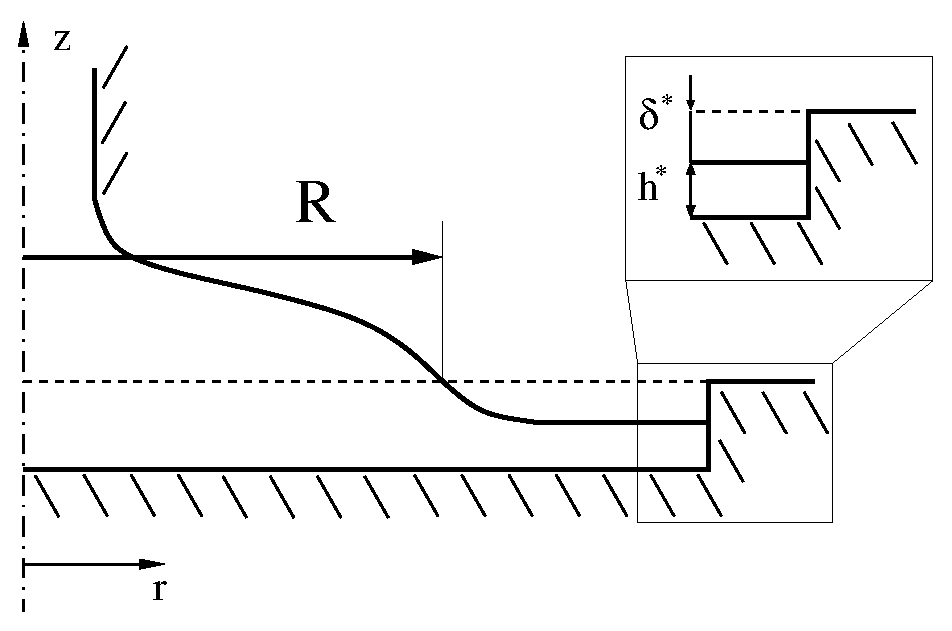
\includegraphics[width=0.4\textwidth]{figures/axisym_drop_nozzle_gap.eps}
\caption{Schematic diagram of the underfilled trough.}
\label{fig:axisym_drop_nozzle_gap}
\end{figure}
 
However, the glucose syrup adhered to the scraper because of the high viscosity of the material, resulting in excess removal of fluid during the scraping process. 
This led to an underfilled trough with a gap height $\delta^*$ between the top surface of the layer and the platform edge, as illustrated in figure \ref{fig:axisym_drop_nozzle_gap}.
Consequently, the actual thickness of the layer, $h^*$, was smaller than the depth of the trough, so that the line of contact between the syrup drop and layer was not visible in the acquired images. 
Hence, the measured radii $R$ quantify the radii at the level of the platform edge and not at the drop-layer contact line.
 
{\renewcommand{\arraystretch}{1.2}
 \begin{table}[!ht]
 \begin{center}
 \begin{tabular}{c | c | c}
  Experiment & Gap $\delta^*$ in mm & Layer thickness $h^*$ in mm \\ 
   \hline
   1) & $1.18 \pm 0.05$ & $0.82 \pm 0.05$ \\
   2) & $1.15 \pm 0.07$ & $0.85 \pm 0.07$
 \end{tabular}
 \caption{Estimated gap sizes $\delta^*$ and layer thicknesses $h^*$ for the different experiments.}
 \label{tab:gap_sizes}
 \end{center}
 \end{table}}
 
The size of the gap was estimated before each experiment by placing a reference object across the underfilled trough to visualise the height of the gap and capturing a side-view image.
Based on these images the gap size was estimated for the two experiments as shown in table \ref{tab:gap_sizes}.
The gap was of similar height in both experiments.

\subsubsection{Image analysis}

We analysed the acquired images using \textit{OpenCV} \cite{bradski2008learning} within a \textit{python} environment. 
In order to convert the results from the image analysis into dimensional quantities, we took a reference image of a cylindrical object, with known height $H^*=10.08$ mm and diameter $D^*=37.32$ mm. 
We placed the object in the centre of the trough so that its effective height was reduced to $H^*_{\sym{eff}}=8.08$ mm.
Small misalignment of the camera can result in images where the platform edge is not parallel to the image edge. 
We corrected this misalignment in post-processing by rotating the image prior to the analysis.
For this purpose we determined the position of the platform edge on the left and right ends of the image. 
We achieved this by sampling the intensities of the grey scale image along a vertical line from top to bottom, resulting in an intensity profile with a smooth step change at the platform edge.
We fitted a tanh-function to the intensity profile, which enabled a sub-pixel resolution.
The difference between the platform position on the left and right is an estimate of the image rotation.
We determined the diameter $D$ of the reference object in pixels by locating its left and right edges with sub-pixel resolution using the same approach for determining the platform edge. 
Similarly, we determined the height of the object $H$ in pixels by locating its upper edge with sub-pixel resolution.
We calculated the relationship between dimensional sizes and corresponding pixel values as $D^*/D$ and $H^*_{\sym{eff}}/H$. 
We chose the actual scaling as the average of these diameter and height relationships and found it to be $0.111 \pm 0.006$ mm/pixel.
We stored this scaling and the image rotation in a file, which we used during the image analysis of the experimental image sequences. \\


We recorded the spreading of a sessile drop of glucose syrup on a layer of the same fluid as a sequence of images, capturing the behaviour from the initial deposition until the drop reached a quasi-equilibrium configuration. 
However, only part of this sequence was analysed. 
We used a slight motion of the syringe nozzle during deposition to determine the first image after the nozzle came to rest as the initial frame.
We chose the final frame to include a duration of 15 s of spreading. 
This was just before the drop pinched off, where it was difficult to track the interface because of reflections at the surface.
We calculated the actual frame rate from the skip count with which the images were aquired, and read the scaling and image rotation angle from a calibration file, as detailed above. 
We detected the position of the platform edge, and the outside diameter of the syringe nozzle and the positions of its left and right edges from the first image of the sequence. 
We achieved this by using a routine to find edges, which samples the intensities along a line, similar to the edge finding routine described above.
However, as the drop spreads the intensity variability increases due to reflections on the fluid surface. 
Hence, the intensity profile ceases to feature a smooth step change as in the case of the reference object, but rather shows continuous variation. 
Therefore we fitted a spline, instead of a tanh-function to this intensity profile.
We then determined the edge with sub-pixel resolution by detecting the point along the spline with maximum gradient. 
We chose the outside diameter of the syringe nozzle as the reference length scale, which we found equal to 9.22 mm from using both calipers and image analysis. 

\begin{figure}[!ht]
\centering
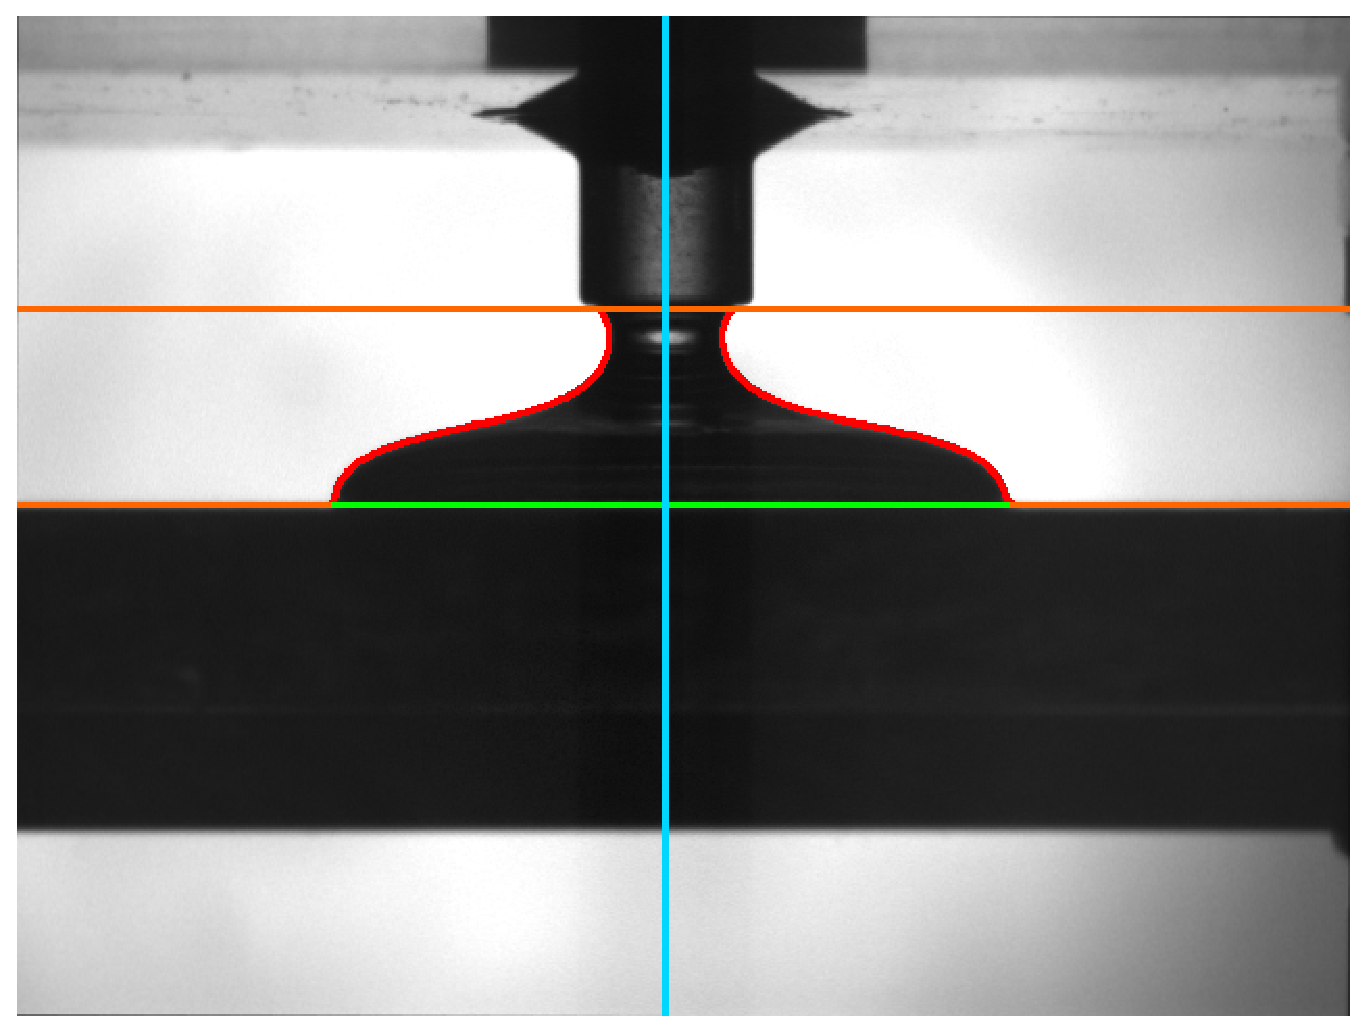
\includegraphics[trim={10px 150px 10px 75px},clip,width=0.5\textwidth]{figures/111014_glucose_syrup_thick_layer_8_0117_analysed.eps}
\caption{Analysed quantities in the glucose experiments: the platform edge and nozzle end, centre line, drop diameter and free surface.}
\label{fig:analysis_glucose}
\end{figure}

We obtained the vertical centre line of the nozzle from the positions of its left and right edges. 
We assumed this to be the centre line of spreading and it is shown in figure \ref{fig:analysis_glucose}. 
We identified the lower edge of the nozzle, and cropped the images to the region between the platform edge and the nozzle end, denoted with horizontal lines in figure \ref{fig:analysis_glucose}. 
We detected the location of the fluid interface to the left and right of the vertical centre line using the same spline-based edge finding routine described above.
As the drop spread, the edge of the interface became less distinct due to surface reflections, in which case the routine failed to detect the free surface location accurately.
In order to improve the robustness of the analysis, we detected the fluid interface based on the interface position in the previous frame of the sequence.
Hence, for subsequent images after the initial frame we applied the edge finding routine to a region of $\pm$ 5 pixels horizontally and $\pm$ 2 pixels vertically of the previously detected location.
We documented the coordinates of the fluid interface separately for the left and right sides, relative to the vertical centre line.
We chose the origin of the coordinate system as the vertical centre line and the platform edge, for the horizontal and vertical coordinates, respectively.


Based on the fluid interface coordinates, we computed the projected area and volume for the regions on the left and right of the vertical centre line separately.
As a measure for the extent of spreading, we recorded the radius of the drop at the level of the platform edge on the left and right, relative to the vertical centre line. 
The error arising in the radii and position of the free surface was the distance to the furthest pixel boundary, in the case of sub-pixel resolution, or one pixel if the determined position was on a pixel boundary.


\subsection{Experimental results}

\subsubsection{Spreading on a layer}
\label{sec:expt_spreading_on_layer}

\begin{figure}[!ht]
 \captionsetup[subfloat]{position=top,singlelinecheck=false, margin=-0.5cm, justification=raggedright}
 \centering
 \subfloat[\label{fig:111014_glucose_syrup_thick_layer_8_0067}]{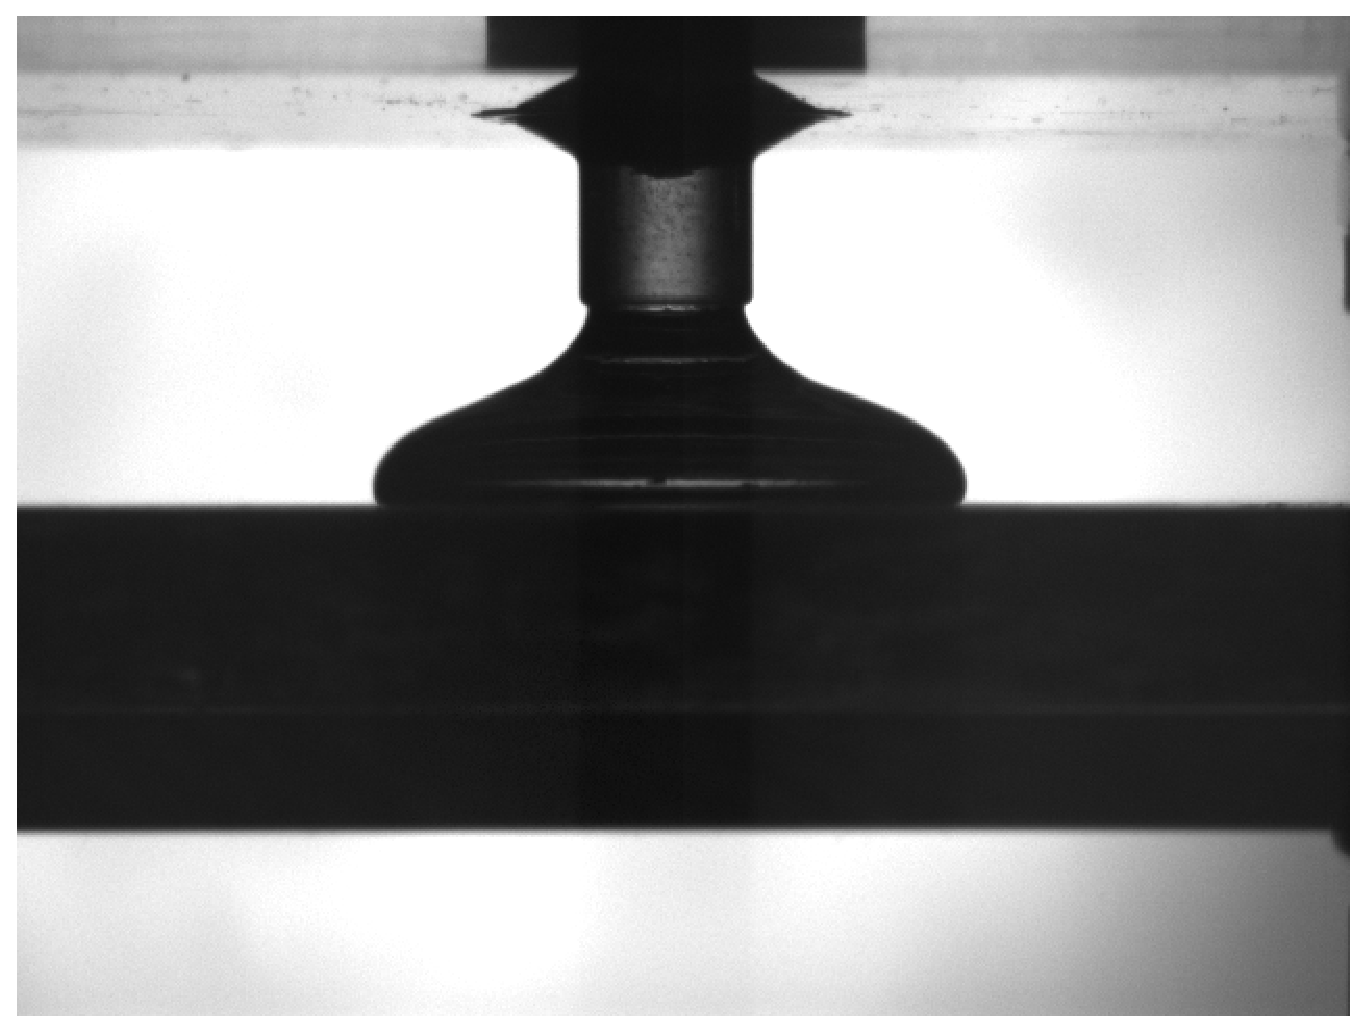
\includegraphics[trim={10px 150px 10px 75px},clip,width=0.2\textwidth]{figures/111014_glucose_syrup_thick_layer_8_0067.eps}} \hspace{0.5cm}
 \subfloat[\label{fig:111014_glucose_syrup_thick_layer_8_0067_analysed}]{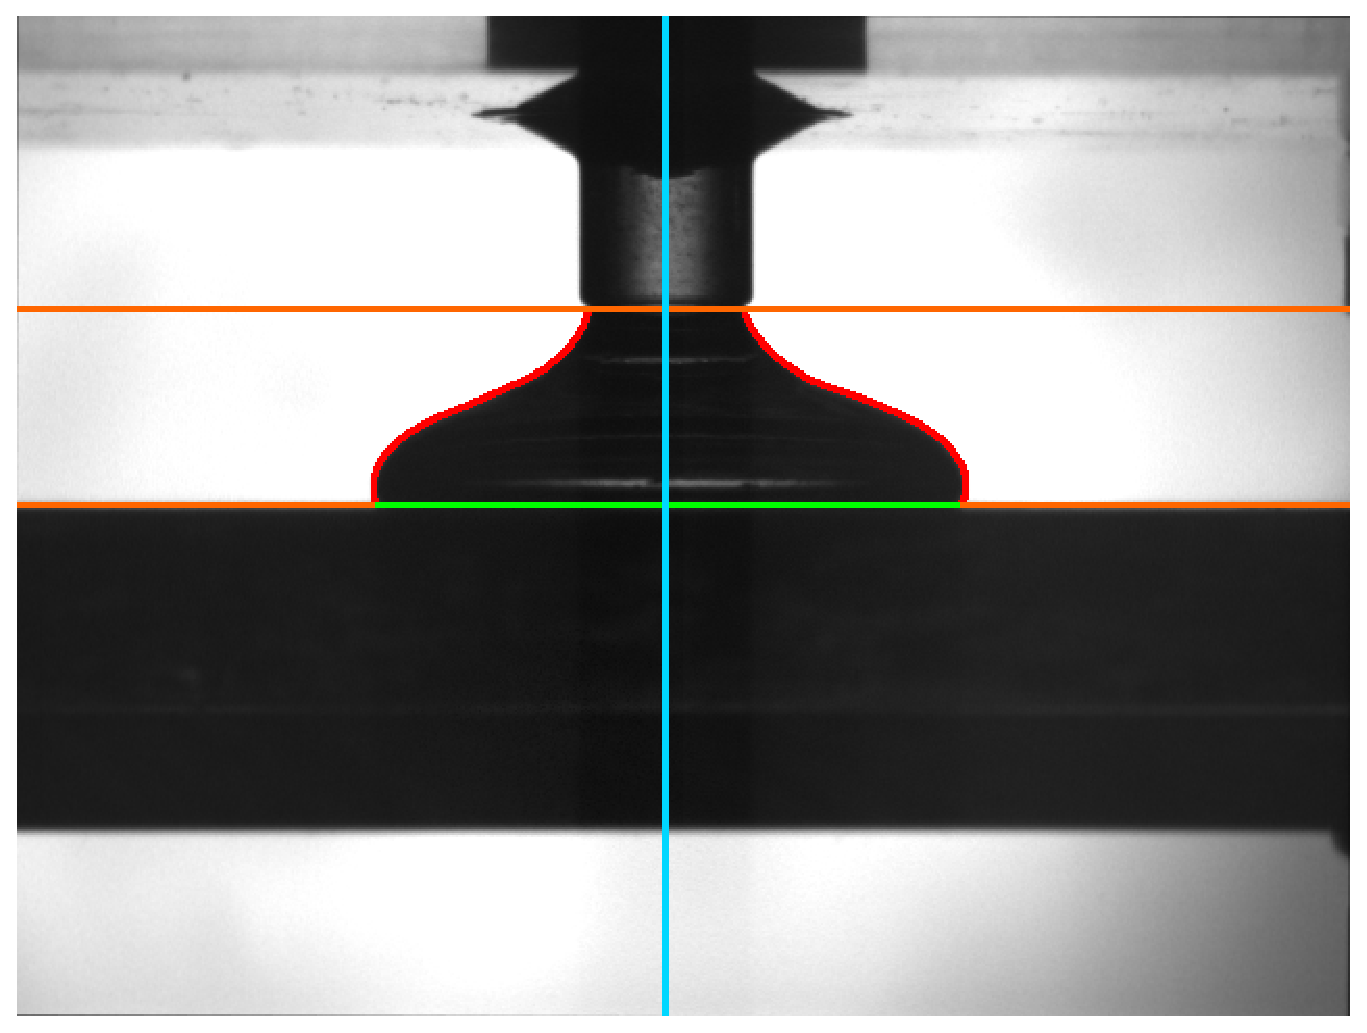
\includegraphics[trim={10px 150px 10px 75px},clip,width=0.2\textwidth]{figures/111014_glucose_syrup_thick_layer_8_0067_analysed.eps}} \\
 \subfloat[\label{fig:111014_glucose_syrup_thick_layer_8_0117}]{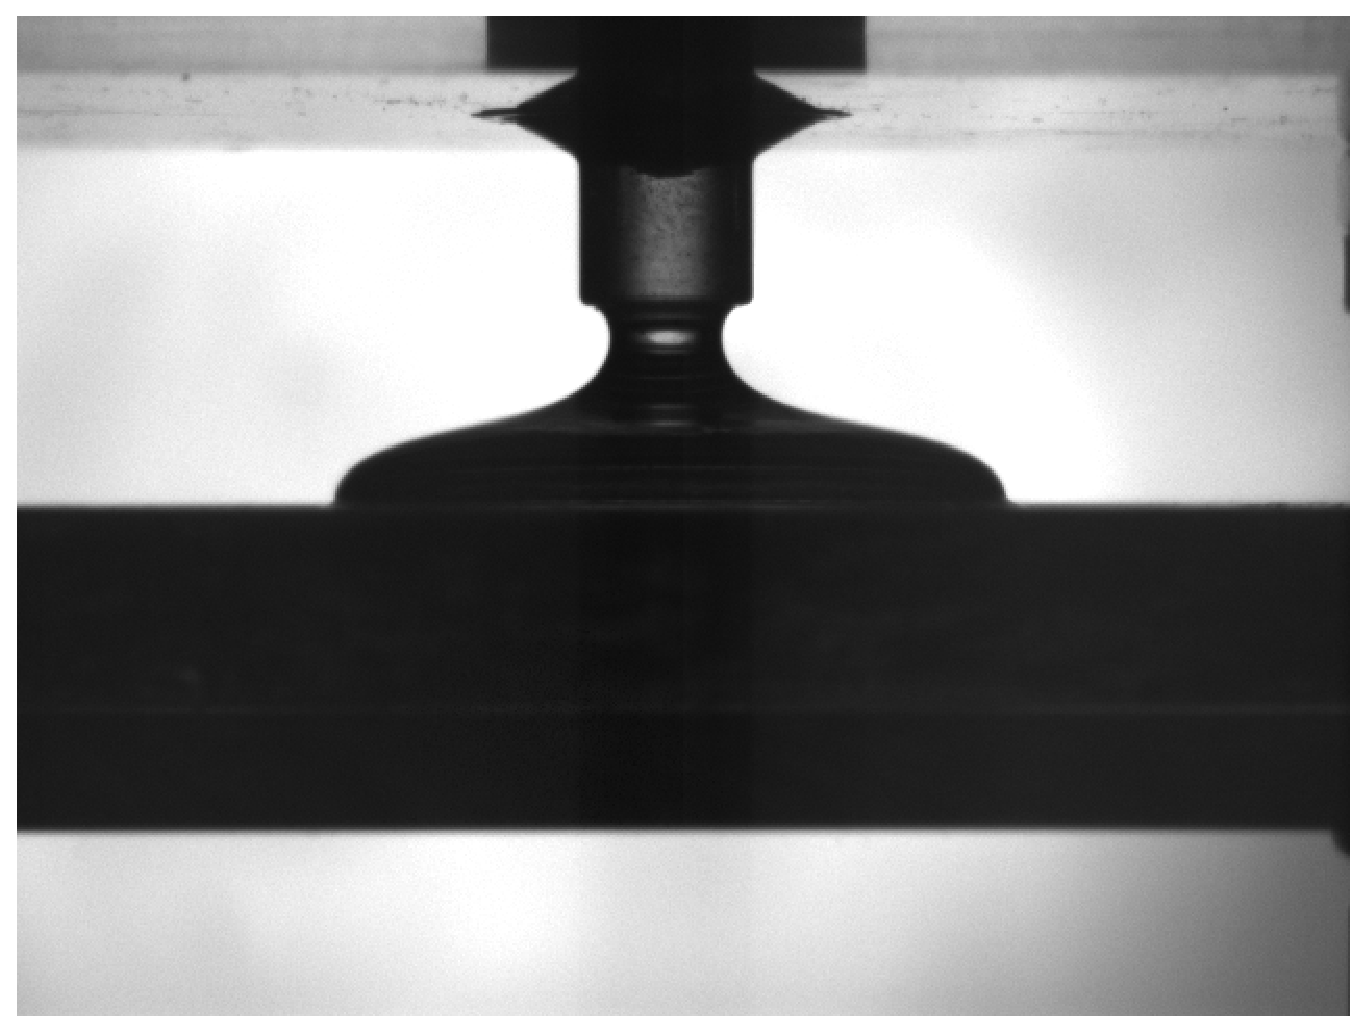
\includegraphics[trim={10px 150px 10px 75px},clip,width=0.2\textwidth]{figures/111014_glucose_syrup_thick_layer_8_0117.eps}} \hspace{0.5cm}
 \subfloat[\label{fig:111014_glucose_syrup_thick_layer_8_0117_analysed}]{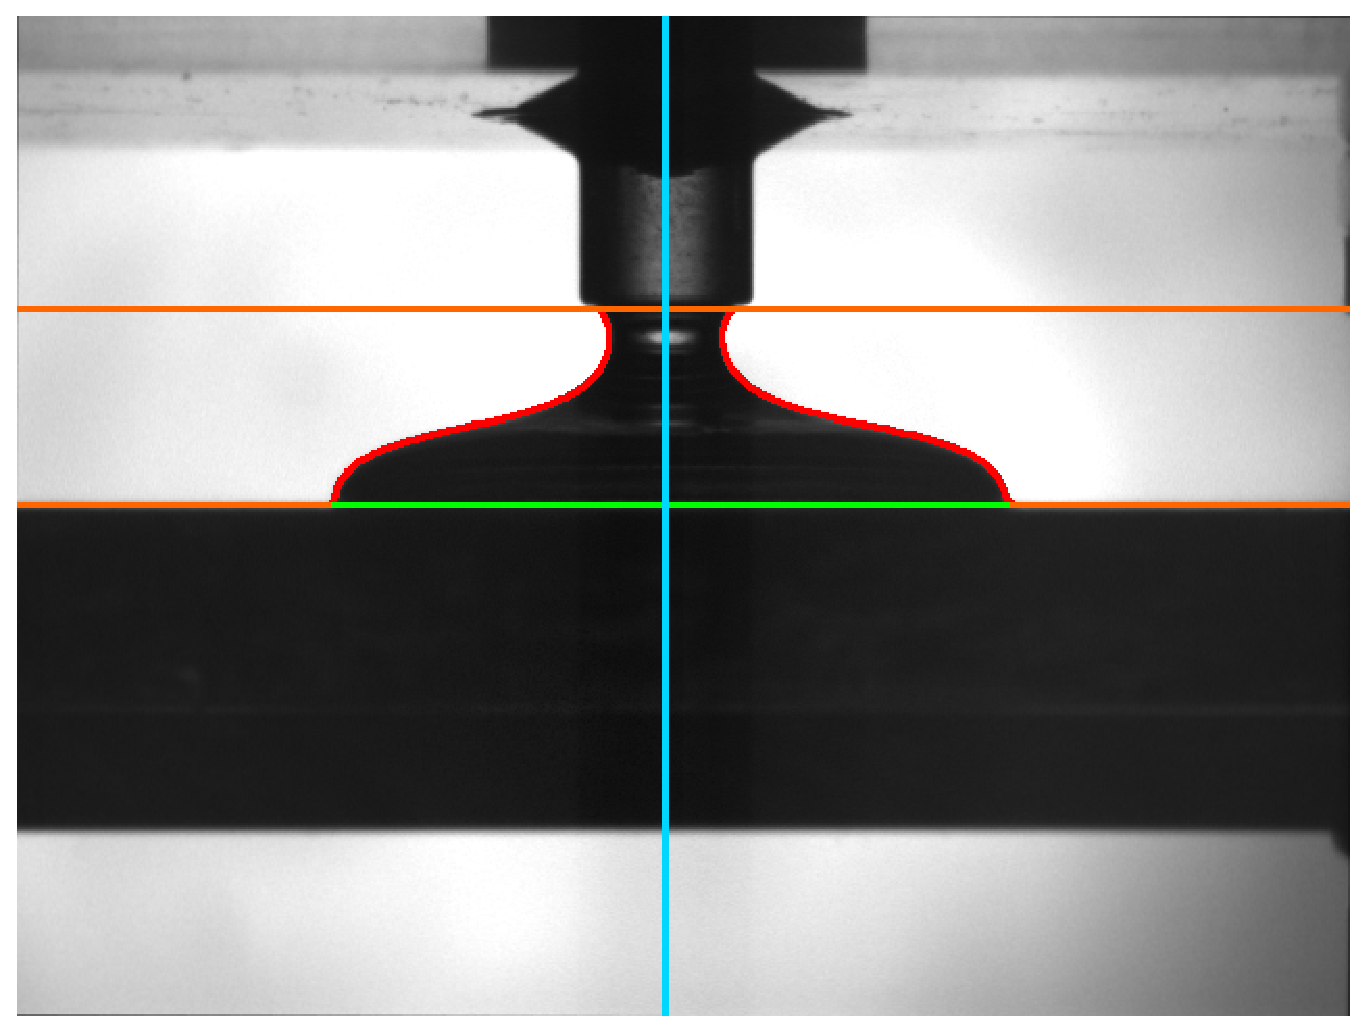
\includegraphics[trim={10px 150px 10px 75px},clip,width=0.2\textwidth]{figures/111014_glucose_syrup_thick_layer_8_0117_analysed.eps}} \\
 \subfloat[\label{fig:111014_glucose_syrup_thick_layer_8_0167}]{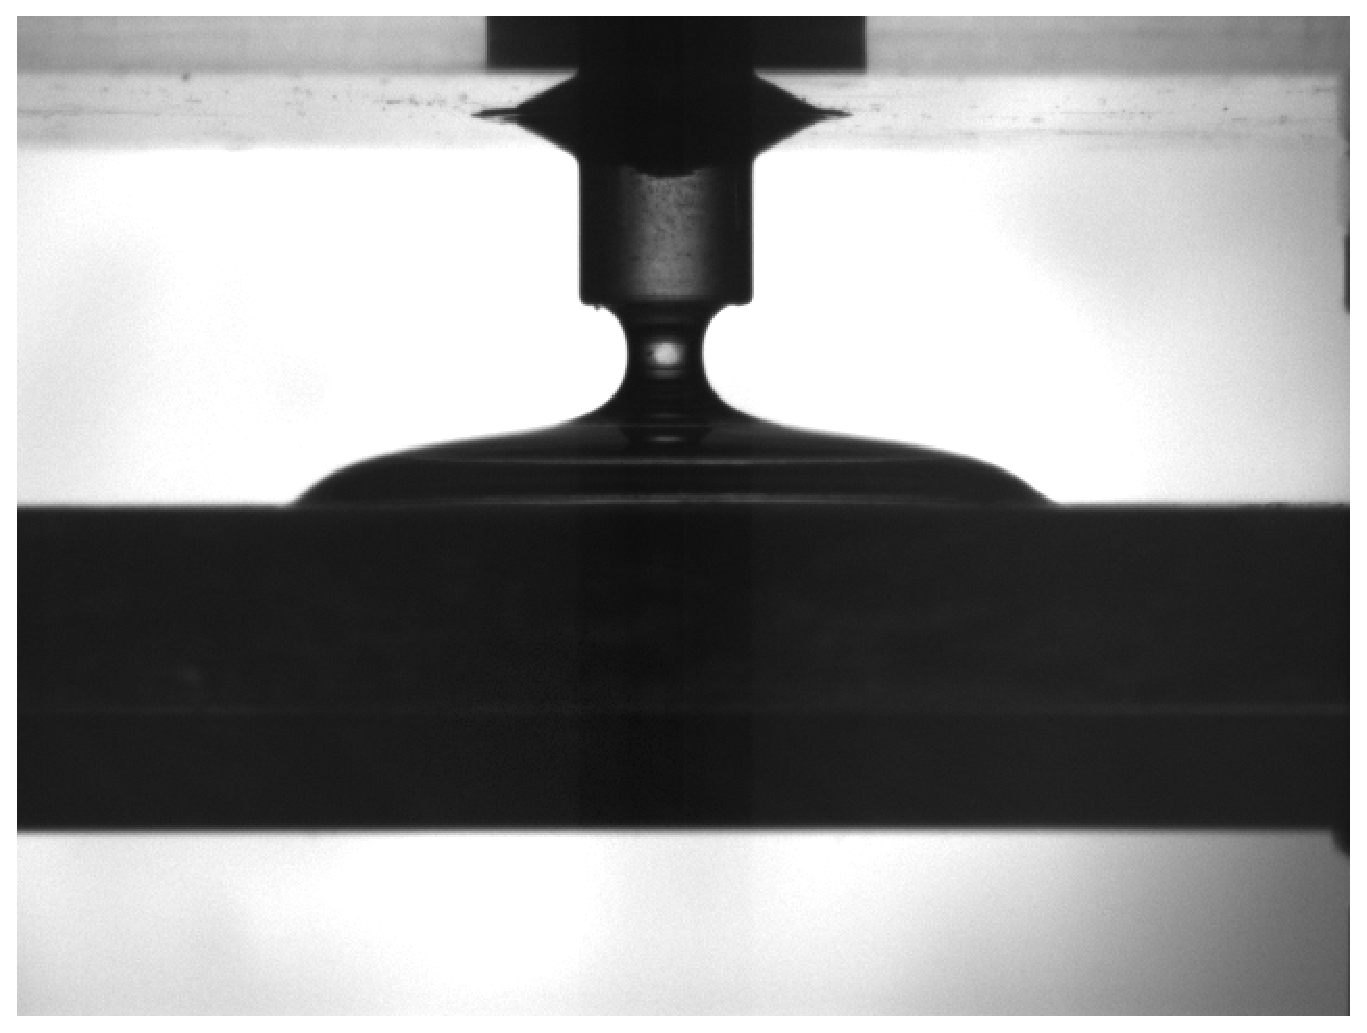
\includegraphics[trim={10px 150px 10px 75px},clip,width=0.2\textwidth]{figures/111014_glucose_syrup_thick_layer_8_0167.eps}} \hspace{0.5cm}
 \subfloat[\label{fig:111014_glucose_syrup_thick_layer_8_0167_analysed}]{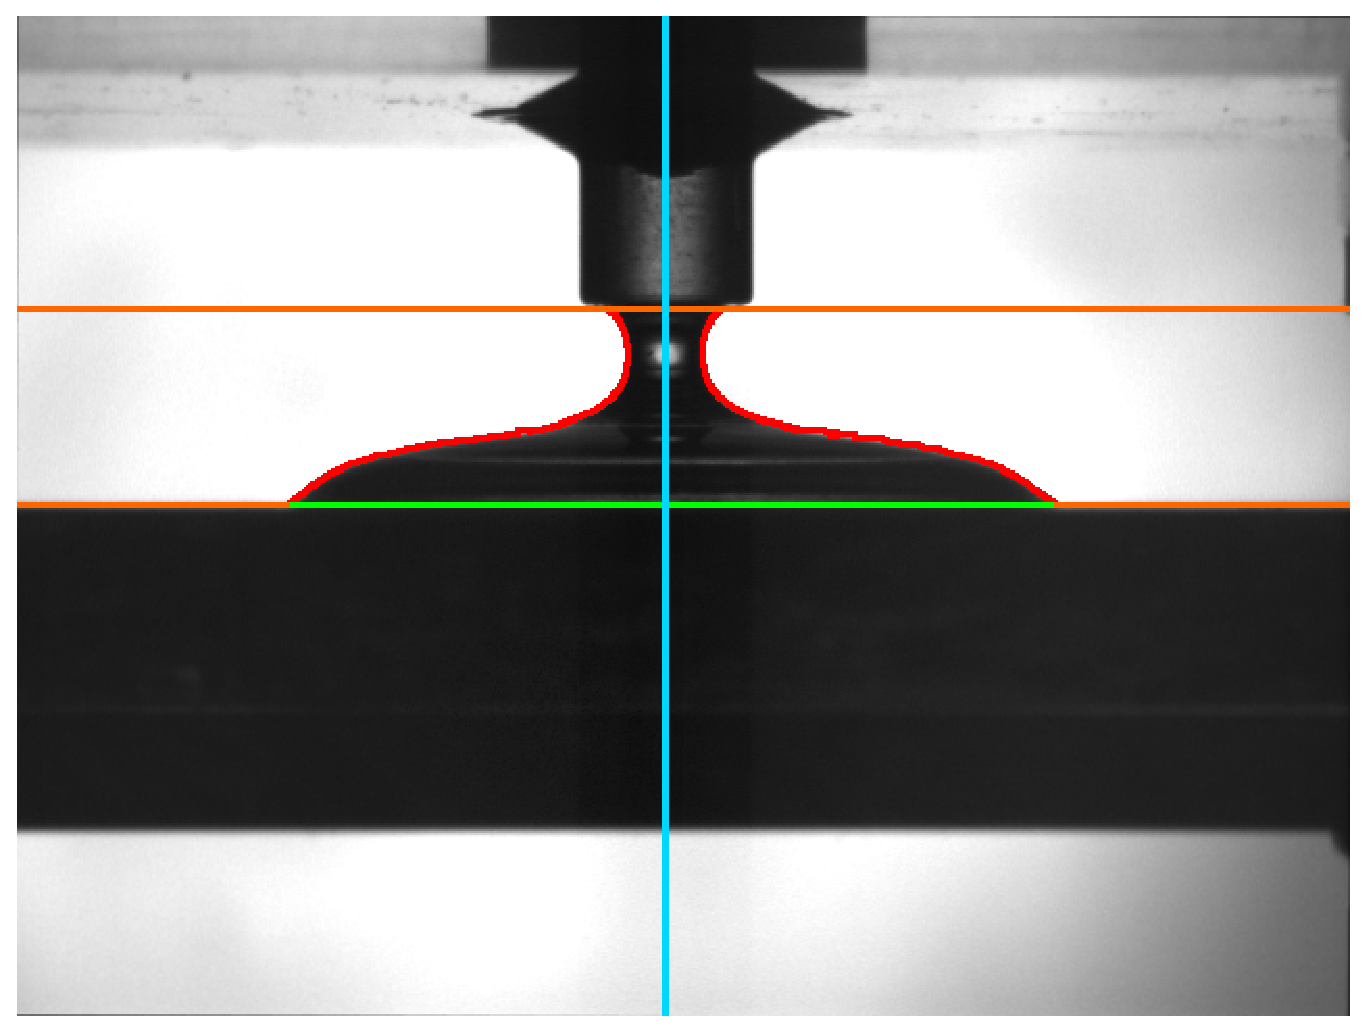
\includegraphics[trim={10px 150px 10px 75px},clip,width=0.2\textwidth]{figures/111014_glucose_syrup_thick_layer_8_0167_analysed.eps}} \\
 \subfloat[\label{fig:111014_glucose_syrup_thick_layer_8_0367}]{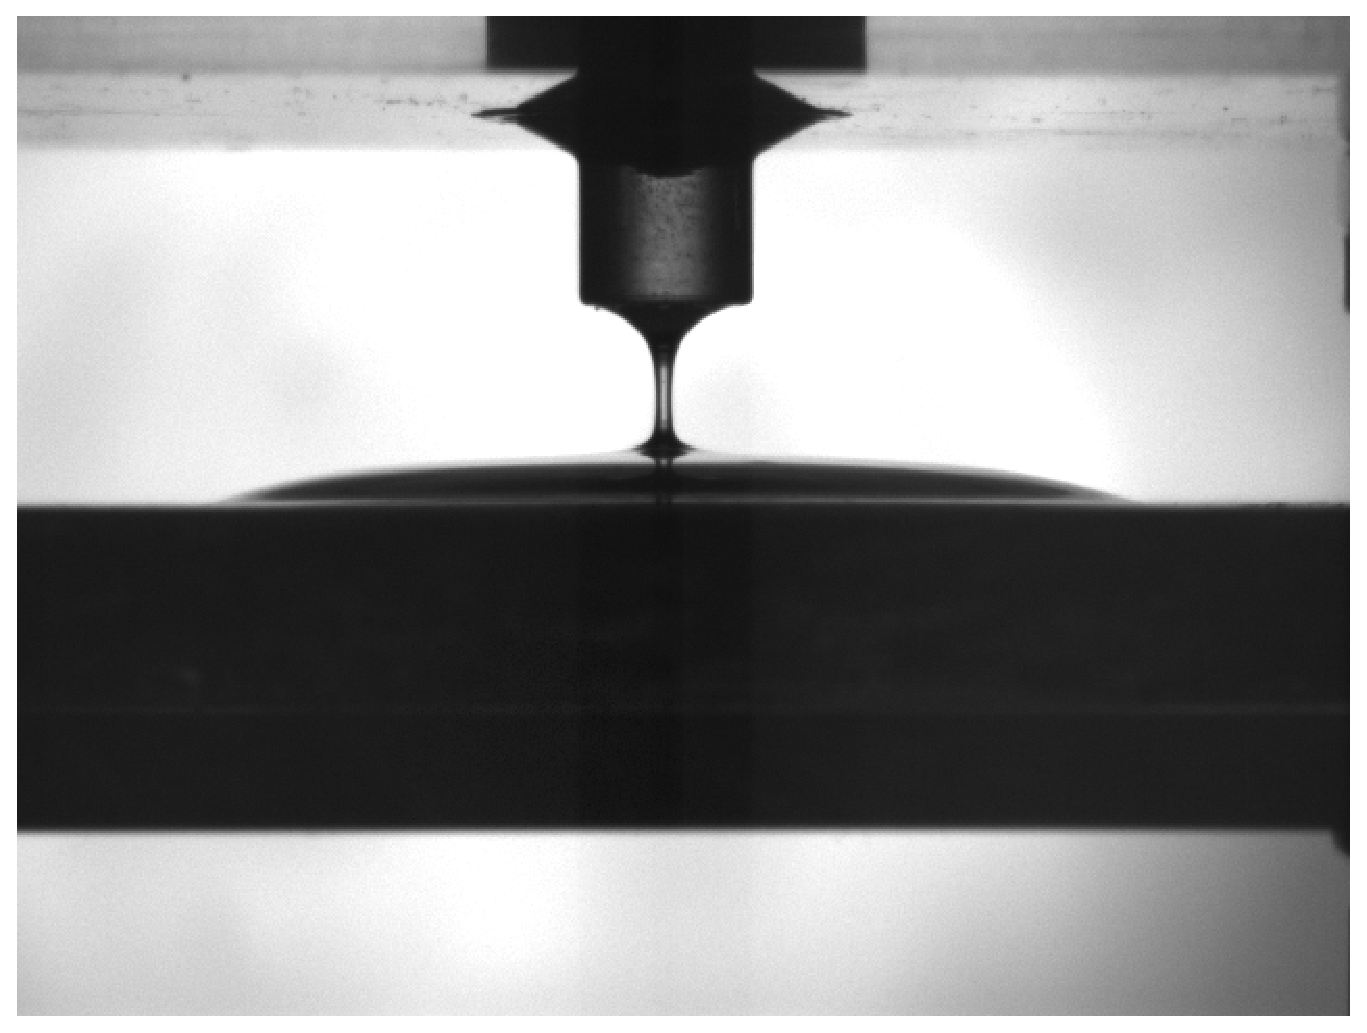
\includegraphics[trim={10px 150px 10px 75px},clip,width=0.2\textwidth]{figures/111014_glucose_syrup_thick_layer_8_0367.eps}} \hspace{0.5cm}
 \subfloat[\label{fig:111014_glucose_syrup_thick_layer_8_0367_analysed}]{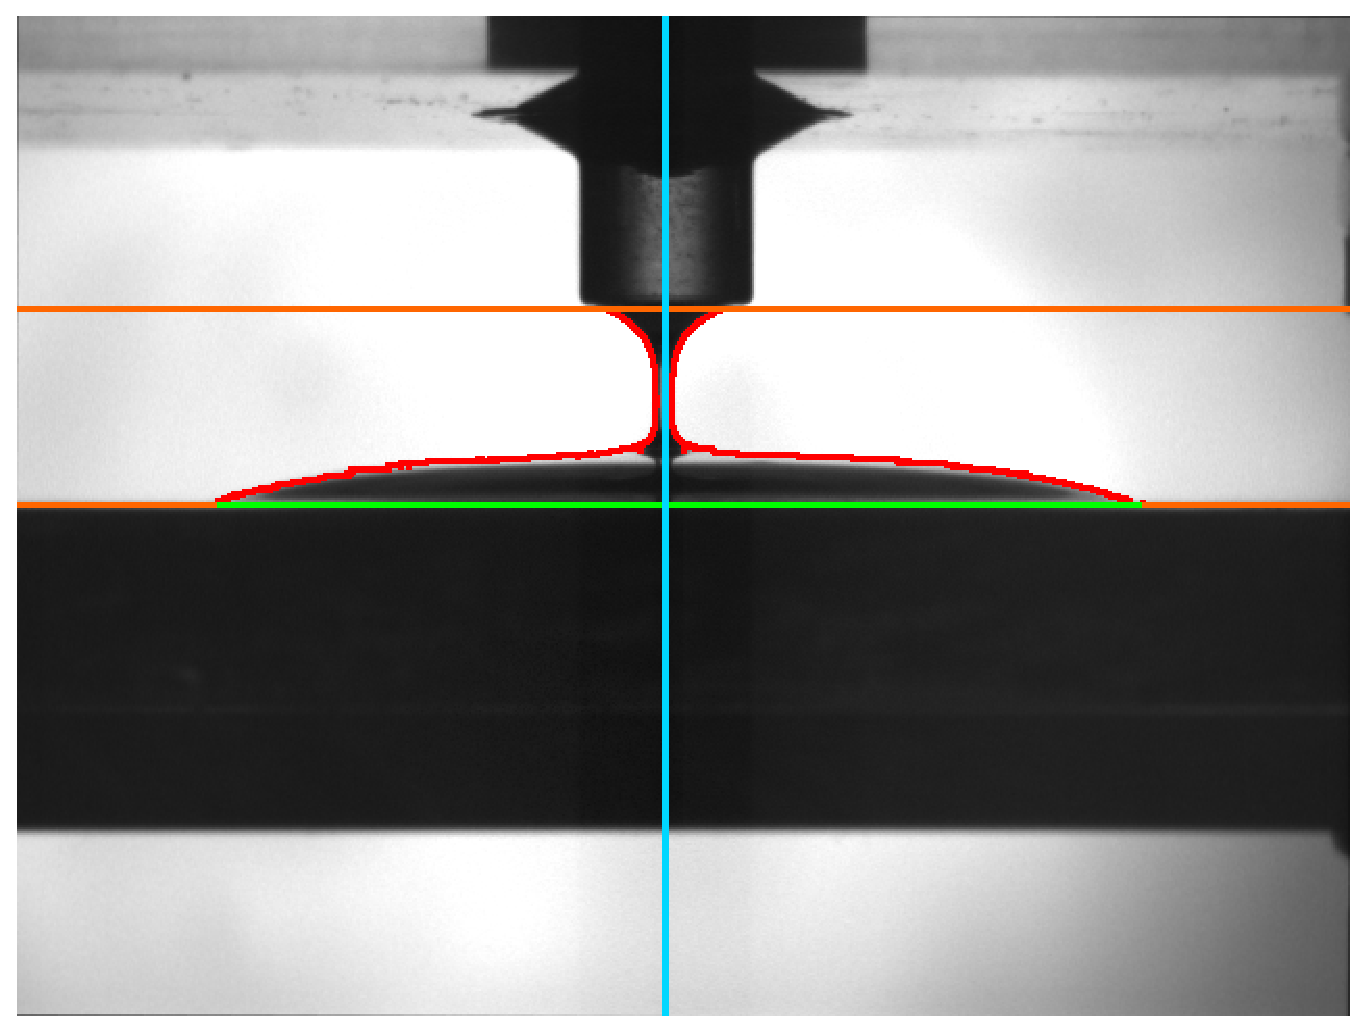
\includegraphics[trim={10px 150px 10px 75px},clip,width=0.2\textwidth]{figures/111014_glucose_syrup_thick_layer_8_0367_analysed.eps}}
  \caption{Side-view images of glucose syrup spreading on a layer of the same fluid at different times for a single experiment: (a)/(b) $t=0.0$ s, (c)/(d) $t=2.5$ s, (e)/(f) $t=5.0$ s, (g)/(h) $t=15.0$ s. Left: rotated and cropped images. Right: processed images, showing the platform edge and nozzle end, centre line, bottom diameter and free surface.\label{fig:glucose_spreading}}
\end{figure}

Selected images of the spreading process recorded during a single experiment are shown in figure \ref{fig:glucose_spreading}. 
The images on the left have been rotated and cropped, but are yet unprocessed. 
The region of interest between the platform edge and the lower edge of the nozzle, is highlighted in the images on the right, together with the vertical centre line. 
These features remain constant throughout the spreading, while the analysed quantities, diameter and free surface shape, change.

\begin{figure}[!ht]
\centering
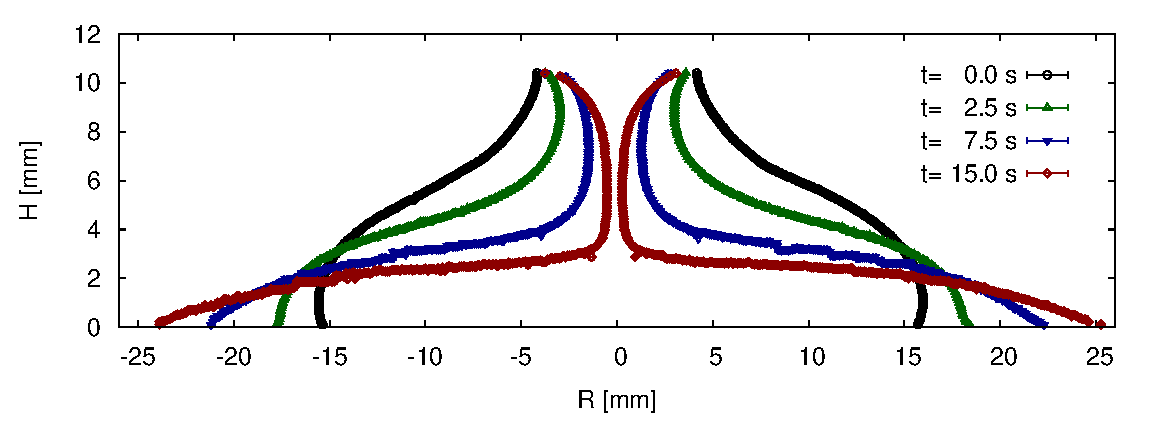
\includegraphics[width=0.9\textwidth]{figures/glucose_thick_layer_8_fs_dim.eps}
\caption{Free surface extracted for a single experiment at different times $t$.}
\label{fig:glucose_thick_layer_8_fs_dim}
\end{figure}

The shape of the free surfaces extracted from the images in figure \ref{fig:glucose_spreading} are shown in a single plot in figure \ref{fig:glucose_thick_layer_8_fs_dim}. 
The initial shape is not perfectly symmetric about the centre line, with a 2 \% larger drop radius on the right than on the left. 
This might be due either to small imperfections in the deposition process or in the levelling of the platform.
Moreover, volume is not conserved in the drop outlines shown in figure \ref{fig:glucose_thick_layer_8_fs_dim}, because fluid spreads below the visible platform edge, as shown schematically in figure \ref{fig:axisym_drop_nozzle_gap}.
The drop shape changes significantly within the first 7.5 s, but only slightly during the following 7.5 s.

\begin{figure}[!ht]
\centering
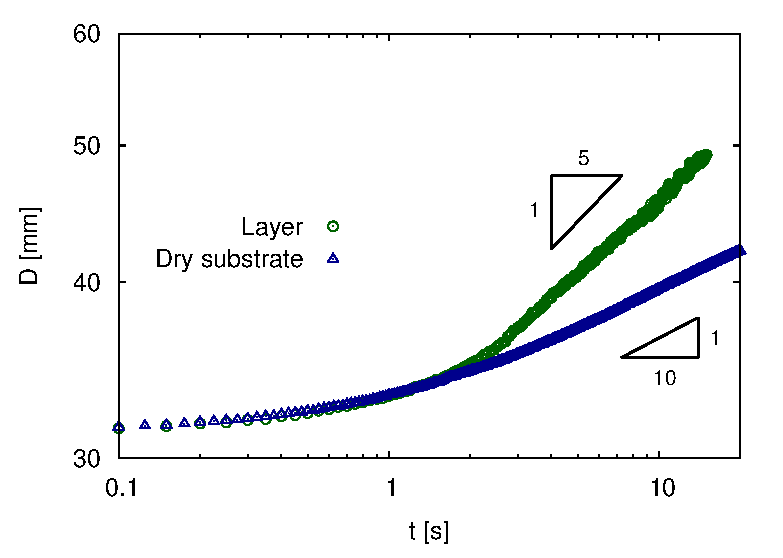
\includegraphics[width=0.6\textwidth]{figures/diam_vs_time_comp_layer_dry.eps}
\caption{Mean diameter evolution across multiple experiments, for spreading on a layer of fluid and on dry substrate, on a log-log scale. Comparison with spreading laws $D \propto t^{1/5}$ and $D \propto t^{1/10}$.}
\label{fig:diam_vs_time_comp_layer_dry}
\end{figure}

The diameter evolution averaged across two experiments is shown in figure \ref{fig:diam_vs_time_comp_layer_dry} on a log-log scale, where the error bars of maximum 1 \% have been omitted for clarity.
Also shown in figure \ref{fig:diam_vs_time_comp_layer_dry} is the spreading law $D \propto t^n$ with a scaling exponent of $n$=1/5. 
This is the theoretical exponent which corresponds to a droplet spreading in two dimensions, where the driving force is gravity and dissipation occurs in the bulk \cite{bonn2009wetting}.
There is good agreement between the experimental data and this theoretical value, indicating that a competition between gravity and viscous dissipation is governing the flow. 
This balance is expressed in the Galileo number

\begin{equation}
 \sym{Ga} = \frac{g \; \mathcal{L}^3}{\nu^2} = \frac{g \; \rho^2 \; \mathcal{L}^3}{\mu^2},
 \label{eqn:galilei}
\end{equation}
where $g$=9.81 m/s$^2$ is the gravitational acceleration and $\mathcal{L}$ the characteristic length scale, which we chose as the outer nozzle radius, $\mathcal{L}=4.61$ mm.
The two experiments were conducted at laboratory temperatures of 20.2 and $\degC{20.4}$, respectively. 
Hence we used the viscosity $\mu$=43.61 Pa.s determined at $\degC{20.3}$ in equation (\ref{eqn:galilei}). 
Using these material parameters and the characteristic length, equation (\ref{eqn:galilei}) yields a Galileo number of $9.52 \times 10^{-4}$, indicating a viscously dominated flow.


\subsubsection{Spreading on a solid substrate}

In order to investigate the spreading of a sessile glucose syrup drop on a solid surface, we repeated the experiments on a dry perspex substrate instead of a layer of the same fluid.
The diameter evolution averaged across three experiments is shown in figure \ref{fig:diam_vs_time_comp_layer_dry} on a log-log scale, where the error bars of maximum 0.5 \% have been omitted for clarity.
We compare the spreading on a dry substrate against the spreading on a layer, established in the previous section.
Initially the spreading rate is similar, indicated by the close superposition of the two curves.
However, for $t > 2$ s the spreading rates start to diverge and the drop on the solid substrate spreads significantly slower than the drop on the fluid layer.
Also shown in figure \ref{fig:diam_vs_time_comp_layer_dry} is the spreading law $D \propto t^{1/10}$, which is the theoretical spreading law for a sessile drop spreading in three dimensions, where the driving force is surface tension and dissipation occurs at the contact line \cite{bonn2009wetting, cazabat1986dynamics}.
The good agreement between the experimental data and this theoretical value indicates that in the case of spreading on a solid surface the flow is governed by a competition of surface tension and viscous dissipation.
This balance is expressed in the Capillary number

\begin{equation}
 \sym{Ca} = \frac{\mathcal{U} \; \mu}{\sigma},
 \label{eqn:capillary}
\end{equation}
where $\sigma=55 \times 10^{-3} \; \sym{N/m}$ is the surface tension of glucose syrup and $\mathcal{U}=\partial D/ \partial t=0.38 \; \sym{mm/s}$ is the contact line speed.
We derived the speed of the contact line in the regime of quasi-steady spreading, for $t > 2$ s, from the spreading law.
With these values equation (\ref{eqn:capillary}) yields a Capillary number of 0.3, indicating that during the spreading of a glucose drop on a solid substrate surface tension effects are more dominant than viscous dissipation.
%Another relevant non-dimensional number is the Bond number, which expresses the balance between gravitational forces and surface tension.
%The Bond number is defined as
%
%\begin{equation}
% \sym{Bo} = \frac{\mathcal{L}^2 \: g \: \Delta \rho}{\sigma},
%\end{equation}
%where $\Delta \rho = (\rho_{\sym{glucose}} - \rho_{\sym{air}})$ is the density difference between the glucose syrup and the surrounding air.
%We make the assumption $\Delta \rho = \rho_{\sym{glucose}}$, because $\rho_{\sym{air}} \ll \rho_{\sym{glucose}}$.
%Substituting for the material properties and reference length yields $\sym{Bo}=5.2$, indicating that the spreading is relatively unaffected by surface tension and instead gravity is more dominant.

\section{Computations}

\subsection{Computational model}

\subsubsection{Governing equations}

We modelled the spreading of a sessile drop of Newtonian glucose syrup spreading on a layer of the same fluid as a flow which is governed by the dimensional, incompressible Navier-Stokes equations,

\begin{equation}
 \rho \Bigg( \pder[\vect{u}^*]{t^*} + (\vect{u}^* \cdot \nabla^*) \vect{u}^* \Bigg) = \rho \vect{G}^* - \nabla^* p^* + \mu \nabla^{*2} \vect{u}^*,
 \label{eqn:ns_eqn_momentum}
\end{equation}
and

\begin{equation}
 \nabla^* \cdot \vect{u}^* = 0,
 \label{eqn:ns_eqn_continuity}
\end{equation}
where $\vect{u}^*$ is the flow velocity vector, $\rho$ the fluid density and $p^*$ the pressure field in the fluid. 
The gravitational body force, per unit volume, is expressed in the vector $\rho \vect{G}^*$. 

We non-dimensionalised equations (\ref{eqn:ns_eqn_momentum}) and (\ref{eqn:ns_eqn_continuity}) using a characteristic length scale, $\mathcal{L}$, reference velocity, $\mathcal{U}$, and reference time, $\mathcal{T}$. 
The gravitational forces are scaled on the gravitational acceleration $g$. 
Hence,

\begin{gather}
 \vect{u}^*=\mathcal{U} \vect{u}, \qquad \vect{x}^*=\mathcal{L} \vect{x}, \qquad t^*= \mathcal{T} t, \qquad \vect{G}^*=g \vect{G}, \qquad p^*= \frac{\mathcal{U} \mu}{\mathcal{L}} p,
 \label{eqn:ns_eqn_nondim}
\end{gather}
where the pressure and the gravitational body force have been non-dimensionalised on the viscous scale.
The non-dimensional, incompressible Navier-Stokes equations are then given by

\begin{equation}
 \sym{Re} \Bigg( \sym{St} \pder[\vect{u}]{t} + (\vect{u} \cdot \nabla) \vect{u} \Bigg) = - \nabla p + \frac{\sym{Re}}{\sym{Fr}} \: \vect{G} + \nabla^2 \vect{u},
 \label{eqn:ns_eqn_momentum_nondim}
\end{equation}
and
\begin{equation}
 \nabla \cdot \vect{u} = 0,
 \label{eqn:ns_eqn_continuity_nondim}
\end{equation}
with the dimensionless parameters

\begin{align*}
 \text{Reynolds number:} \qquad &\sym{Re}=\frac{\mathcal{UL} \rho}{\mu}, \\
 \text{Strouhal number:} \qquad &\sym{St}=\frac{\mathcal{L}}{\mathcal{UT}}, \\
 \text{Froude number:} \qquad &\sym{Fr}=\frac{\mathcal{U}^2}{g \mathcal{L}}.
\end{align*}

Equations (\ref{eqn:ns_eqn_momentum_nondim}) and (\ref{eqn:ns_eqn_continuity_nondim}) are used to determine the pressure and velocity field within a certain domain $\mathcal{D}$. 
In order to obtain these fields, the equations have to be augmented by boundary conditions along at least part of the domain boundary $\partial \mathcal{D}$.

\begin{figure}[!ht]
\centering
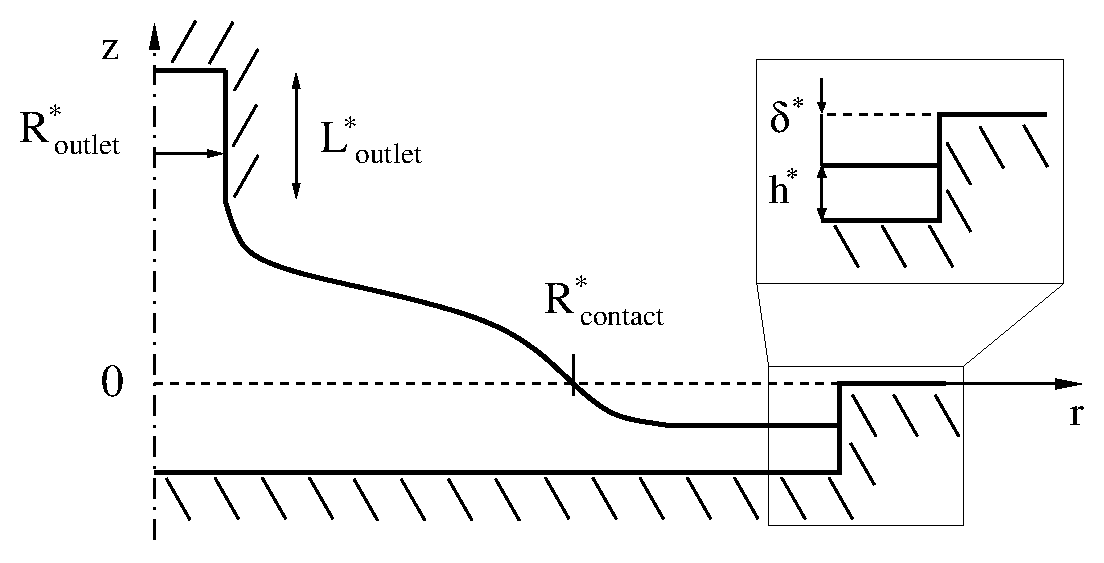
\includegraphics[width=0.6\textwidth]{figures/axisym_drop_nozzle_gap_computation.eps}
\caption{Schematic diagram of a model in cylindrical polar coordinates of the experiment investigating the spreading of a drop on a layer of the same fluid, where $R_{\sym{contact}}(t)=r(t,z=0)$ is the experimentally visible drop radius.}
\label{fig:axisym_drop_nozzle}
\end{figure}

A schematic diagram of the flow domain and the domain boundaries is shown in figure \ref{fig:axisym_drop_nozzle}.
In the experiments the glucose syrup is deposited using a syringe with a widened nozzle outlet.
The residual fluid in this outlet, following deposition, is included in the numerical model, as shown in figure \ref{fig:axisym_drop_nozzle}, where the top boundary represents the plunger of the syringe and the side boundary is the inner radius of the outlet.
The nozzle is $L^*_{\sym{outlet}}=10$ mm long and the inner radius is determined from the highest point on the free surface.
We solved the equations in cylindrical polar coordinates, with the assumption that there is no variation in the azimuthal direction ($\partial / \partial \phi = 0$), so that it becomes an axisymmetric flow problem in the two spatial dimensions $\vect{x}=\{r,z\}$. 
Moreover, we assumed that there is no swirl, $u_{\phi}=0$, so that the velocity field is $\vect{u}=\{u_r,u_z\}$.
Also, the gravitational acceleration is only acting in the axial direction, $G_z = -1$ and $G_i=0, i = \{ r,\phi \}$.
As shown in figure \ref{fig:axisym_drop_nozzle}, we model the bottom and outer wall of the trough, and the top and outer wall of the nozzle as solid walls.
On these boundaries we apply Dirichlet boundary conditions by prescribing the velocity such that the fluid neither penetrates the wall nor 'slips' along it. 
This 'no slip' boundary condition is expressed as

\begin{equation}
 \vect{u}^* = \pder[\vect{R}_{\sym{wall}}^*]{t^*},
 \label{eqn:ns_eqn_solid_wall_bc}
\end{equation}
where $\vect{R}_{\sym{wall}}^*$ is the Lagrangian position of the respective solid boundary. 
All of the solid boundaries in our model remain stationary and hence $\partial \vect{R}_{\sym{wall}}^*/ \partial t^* = 0$.
Therefore, this boundary condition reduces to

\begin{equation}
 \vect{u} = 0,
 \label{eqn:ns_eqn_solid_wall_bc_non_dim}
\end{equation}
in non-dimensional form.

We modelled the centre line of the drop, at $r=0$, as symmetry boundary on which the velocity normal to the boundary and the traction tangential to the boundary is zero. 
These two conditions are mathematically expressed as

\begin{equation}
 \vect{u}^* \cdot \vect{n}_{\sym{sym}} = 0,
\end{equation}
and

\begin{equation}
 \vect{t}^* \cdot \vect{m}_{\sym{sym}} = 0,
\end{equation}
respectively, where $\vect{n}_{\sym{sym}}$ is the unit normal and $\vect{m}_{\sym{sym}}$ is the unit vector tangent to the symmetry line.
The traction on the boundary, which is equivalent to a Neumann boundary condition, is expressed as

\begin{equation}
 \vect{t}^* = \vect{\sigma}^* \cdot \vect{n}_{\sym{sym}}.
 \label{eqn:ns_eqn_solid_wall_traction_bc}
\end{equation}
In the two-dimensional coordinate space $(r,z)$ the normal and tangent to the symmetry boundary are given by $\vect{n}_{\sym{sym}}= (1 \; 0)$ and $\vect{m}_{\sym{sym}} = (0 \; 1)$.
Hence, the two boundary conditions in non-dimensional form become

\begin{equation}
 u_r = 0,
 \label{eqn:ns_eqn_sym_bc_non_dim}
\end{equation}
and

\begin{equation}
 t_z = 0 \quad \text{or} \quad \pder[u_z]{r} = 0.
\end{equation}

At the interface between the glucose syrup and the surrounding atmosphere, as illustrated in figure \ref{fig:axisym_drop_nozzle}, two boundary conditions need to be applied. 
Firstly, at the free surface the traction is not imposed implicitly, but arises from the dynamic boundary condition, which ensures the balance of forces at the free surface. 
Secondly, the kinematic condition links the motion of the fluid interface to the fluid velocities at the interface.


The dynamic boundary condition ensures that the stress is continuous across the interface between two immiscible fluids. 
Now, the traction exerted by fluid 1 onto fluid 2, $\vect{t}^{[1]*}$, is equal but with opposite orientation to the traction exerted by fluid 2 onto fluid 1, $\vect{t}^{[2]*}$ and hence, $\vect{t}^{[1]*} = - \vect{t}^{[2]*}$. 
The traction at the interface in fluid $\beta$ ($\beta=1,2$) is given by

\begin{equation}
 \vect{t}^{[\beta]*} = \vect{\sigma}^{[\beta]*} \cdot \vect{n}^{[\beta]},
\end{equation}
where $\vect{\sigma}^{[\beta]*}$ is the Cauchy stress tensor in fluid $\beta$ and $\vect{n}^{[\beta]}$ is the outer unit normal to fluid $\beta$, pointing out of the fluid. 
Following the definition of the interface normals, $\vect{n}^{[2]} = - \vect{n}^{[1]}$ and hence,

\begin{equation}
 \vect{\sigma}^{[1]*} \cdot \vect{n}^{[1]} = \vect{\sigma}^{[2]*} \cdot \vect{n}^{[1]},
\end{equation}
where we arbitrarily chose the outer unit normal to fluid 1, $\vect{n}^{[1]}$, as the unit normal.


If the interface is curved, surface tension creates a pressure jump across the interface. 
The pressure jump is given by $\Delta p^* = \sigma \kappa^*$, where $\sigma$ is the (constant) surface tension and $\kappa^*$ is twice the mean curvature of the interface and can be calculated from the unit normal to the interface through

\begin{equation}
 \kappa^* = - \nabla_S^* \cdot \vect{n}^{[1]},
\end{equation}
where $\nabla_S^*$ is the surface gradient. 
For the dynamic boundary condition follows

\begin{equation}
 \vect{\sigma}^{[1]*} \cdot \vect{n}^{[1]} = \vect{\sigma}^{[2]*} \cdot \vect{n}^{[1]} + \sigma \kappa^* \vect{n}^{[1]},
\end{equation}
where $\kappa^* < 0$ if the centre of curvature lies inside fluid 1.
Using the reference quantities from (\ref{eqn:ns_eqn_nondim})

\begin{equation}
 \vect{\sigma}^*= \frac{\mathcal{U} \mu_{\sym{ref}}}{\mathcal{L}} \vect{\sigma} \qquad \text{and} \qquad \kappa^*= \frac{1}{\mathcal{L}} \kappa,
\end{equation}
the non-dimensional form of the dynamic boundary condition is given by

\begin{equation}
 \vect{\sigma}^{[1]} \cdot \vect{n}^{[1]} = \vect{\sigma}^{[2]} \cdot \vect{n}^{[1]} + \frac{1}{\sym{Ca}} \kappa \vect{n}^{[1]},
\end{equation}
where the Capillary number is defined as

\begin{equation}
 \sym{Ca} = \frac{\mathcal{U} \mu}{\sigma}.
\end{equation}
We assume that fluid 2 is an inviscid gas so that its stress tensor reduces to $\vect{\sigma}^{[2]}=-p_{\sym{ext}} \: \vect{I}$, where $p_{\sym{ext}}$ is the (non-dimensional) constant pressure above the free surface. 
In this case the non-dimensional dynamic boundary condition becomes

\begin{equation}
 \vect{\sigma} \cdot \vect{n} = \frac{1}{\sym{Ca}} \kappa \vect{n} - p_{\sym{ext}} \vect{n},
 \label{eqn:ns_eqn_dynamic_fs_bc_non_dim}
\end{equation}
where the explicit references to fluid 1 have been dropped, as it is understood that in this specific case the stress tensor and unit normal refer to the single viscous fluid present in the problem.

The kinematic condition ensures that the fluid particles at the free surface remain there at all times. 
If the free surface is parametrised by the intrinsic coordinates $\vect{\zeta}^*$, then the Eulerian position of the free surface at any given time is written as $\vect{R}_{\sym{fs}}^*=\vect{R}_{\sym{fs}}^*(\vect{\zeta}^*,t^*)$.
The kinematic condition is then given by

\begin{equation}
 \Bigg( \vect{u}^* - \pder[\vect{R}_{\sym{fs}}^*]{t^*} \Bigg) \cdot \vect{n} = 0,
\end{equation}
where $\vect{n}$ is the outer unit normal to the free surface, pointing out of the fluid. 
Using the problem-specific quantities from (\ref{eqn:ns_eqn_nondim}) and using the non-dimensionalisations

\begin{equation}
 \vect{u}^* = \mathcal{U} \vect{u}, \qquad \vect{R}_{\sym{fs}}^* = \mathcal{L} \vect{R}_{\sym{fs}} \qquad \text{and} \qquad t^*=\mathcal{T} t,
\end{equation}
the non-dimensional form of the kinematic boundary condition becomes

\begin{equation}
 \Bigg( \vect{u} - \sym{St} \: \pder[\vect{R}_{\sym{fs}}]{t} \Bigg) \cdot \vect{n} = 0.
 \label{eqn:ns_eqn_kinematic_fs_bc_non_dim}
\end{equation}



In order to validate the computations against the experimentally observed flow, we numerically modelled the single spreading experiment on a layer as presented in section \ref{sec:expt_spreading_on_layer}.
The second experiment for the spreading on a layer is qualitatively similar and is therefore not specifically discussed here.
The initial shape of the free surface in the computation is constructed based on the free surface location determined during the experimental analysis.
However, the computation is limited to one side of the free surface, because axisymmetric flow is assumed and we arbitrarily chose the right-hand surface of the drop.
As discussed in section \ref{sec:creating_layer} we found experimentally that there is a gap $\delta^*$ between the fluid layer and platform edge which means that part of the drop surface is invisible in the experiment, as indicated in figure \ref{fig:axisym_drop_nozzle}.
The size of this gap was difficult to determine accurately and was therefore estimated at $\delta^*=1.15$ mm, resulting in an estimated uniform fluid layer thickness of $h^*=0.85$ mm.
However, through numerical experiments we found that the actual layer thickness was $h^*=1.25$ mm and the results for the estimated and computationally re-constructed layer thickness are compared in section \ref{sec:comp_spreading_on_layer}.
For the flow simulation we re-constructed the experimentally invisible part of the free surface by fitting a spline through the points on the uniform fluid layer and the visible part of the surface.
The quantity $R_{\sym{contact}}^*$ in figure \ref{fig:axisym_drop_nozzle} represents the outermost experimentally visible drop radius at the level of the platform edge, which in the model is located at $z=0$, as indicated in the schematic diagram.

\subsubsection{Non-dimensional parameters}

We chose the outer radius of the nozzle outlet $R_{\sym{outlet}}^*$ as shown in figure \ref{fig:axisym_drop_nozzle} as characteristic length scale, $\mathcal{L}$, in this problem.
As the characteristic velocity scale of the problem we chose the settling velocity of a sessile drop under gravity, so that

\begin{equation}
 \mathcal{U}=\frac{\rho g \mathcal{L}^2}{\mu},
 \label{eqn:vel_scale}
\end{equation}
where $\mu$ and $\rho$ are the glucose viscosity and density, respectively, which we determined experimentally.
We chose the intrinsic timescale as the reference timescale for the setup,

\begin{equation}
 \mathcal{T} = \frac{\mathcal{L}}{\mathcal{U}} = \frac{\mu}{\rho g \mathcal{L}},
 \label{eqn:time_scale}
\end{equation}
resulting in a unit Strouhal number.
In summary, the non-dimensional parameters that enter the Navier-Stokes equations directly are given by

\begin{gather}
 \sym{Re} = \frac{\rho \mathcal{U L}}{\mu} = \frac{\rho^2 \; g \; R_{\sym{outlet}}^{*3}}{\mu^2}, \qquad \sym{St} = \frac{\mathcal{L}}{\mathcal{U} \mathcal{T}} = 1, \qquad \sym{Fr} = \frac{\mathcal{U}^2}{g \; \mathcal{L}} = \frac{\rho^2 \; g \; R_{\sym{outlet}}^{*3}}{\mu^2} = \sym{Re}, \nonumber \\[0.75cm]
 \sym{Ca} = \frac{\mu \mathcal{U}}{\sigma} = \frac{\rho g R_{\sym{outlet}}^{*2}}{\sigma}.
 \label{eqn:nondim_numbers}
\end{gather}
For this choice of non-dimensionalisation, $\sym{Ca}$ is independent of the viscosity and $\sym{Fr}=\sym{Re}$, so that $\sym{Re}/\sym{Fr} = 1$.
We non-dimensionalised the geometric parameters on the reference length scale of the problem such that

\begin{equation}
 h = \frac{h^*}{R_{\sym{outlet}}^*}, \qquad \delta = \frac{\delta^*}{R_{\sym{outlet}}^*}, \qquad R_{\sym{outer}} = \frac{R_{\sym{outer}}^*}{R_{\sym{outlet}}^*}, \qquad L_{\sym{outlet}} = \frac{L_{\sym{outlet}}^*}{R_{\sym{outlet}}^*},
\end{equation}
where $R_{\sym{outer}}^*$ the radius of the trough.
The values of the non-dimensional numbers are

\begin{equation}
 \sym{Re} = \sym{Fr} = 9.523 \times 10^{-4}, \qquad \sym{St}=1, \qquad \sym{Ca}=5.204,
\end{equation}
and the geometric values are

\begin{equation}
 h = 0.184, \qquad \delta=0.249, \qquad R_{\sym{outer}}=6.562, \qquad L_{\sym{outlet}}=2.169.
\end{equation}

\subsubsection{Discretisation in FEM}

We discretised the fluid domain and the domain boundary using the finite element method (FEM) as implemented in \texttt{oomph-lib} \cite{HeilHazelOomph2006}.
Flow problems involving free surfaces are conveniently represented using unstructured meshes with triangular elements, because it is challenging to represent complex interface shapes using structured meshes with a set of rectangular elements.
Therefore, we used triangular elements in an axisymmetric coordinate systems and we generated the unstructured meshes using \texttt{Triangle} \cite{shewchuk96b}.
Specifically, we used six-noded, triangular Taylor-Hood \cite{taylor1973numerical} elements ($P_2 P_1$) with a maximum element area of 0.05.
The Taylor-Hood elements satisfy the Lady\u{z}enskaja-Babu\u{s}ka-Brezzi (LBB) condition \cite{sani2000incompressible}, which means that they do not feature any spurious pressure modes.
Moreover, the solution obtained with these elements is guaranteed to converge at the optimal, quadratic convergence rate under mesh refinement \cite{donea2003finite}.
In the free-surface problem that we modelled, the domain is moving and it is discretised using an unstructured mesh which is fitted to the fluid domain. 
Hence, the mesh is deforming in response to the motion of the fluid, which we realised by using the Arbitrary Lagrangian Eulerian (ALE) method \cite{donea1982arbitrary}.
Specifically, the change of the mesh shape is driven by the motion of the free surface.
Additional unknowns are introduced, because the location of the free surface $\vect{R}_{\sym{fs}}$ is unknown and has to be determined during the solution process.
The additional equations that need to be solved to obtain $\vect{R}_{\sym{fs}}$ arise from the kinematic boundary condition.
At every timestep the location of the free surface is determined and the positions of the nodes in the mesh are updated accordingly employing a pseudo-solid mesh approach.
The pseudo-solid node-update procedure treats the mesh as an elastic body, which deforms, and at every timestep a solid mechanics problem needs to be solved simultaneously with the fluids problem to compute the unknown nodal positions.
The position of the free surface is imposed by artificial pressures acting normal to the interface, which have the function of Lagrange multipliers and are obtained through the solution of the kinematic boundary condition.
Although this approach is computationally expensive as it introduces two additional unknowns at each node and a solid mechanics problem has to be solved at each timestep, it enables the simulation of flows with complex free surface shapes, which is required for our problem.
In the process of timestepping, the elements in the mesh become increasingly distorted, because the node positions are constantly updated.
Therefore we re-generated the mesh after every two time steps based on the current position of the domain boundaries and the current solution is projected across onto the new mesh.
We performed time-dependent simulations and used a second-order accurate Backward Differentiation Formula (BDF2) scheme \cite{sani2000incompressible} for the temporal discretisation.
In order to enable direct comparison with the experiment, the flow was simulated for the duration of the experiment, $t^*_{\sym{exp}}=15$ s.
The time step in the temporal discretisation was chosen as the time difference between successive frames in the experiment, $\Delta t^*_{\sym{exp}} = 0.05$ s.
We performed mesh independence studies, which showed that the chosen spatial and temporal discretisation accurately resolve the problem.
At every time step we recorded the shape of the free surface and the radius $R_{\sym{contact}}(t)=r(t,z=0)$.

\subsection{Computational results}

\subsubsection{Spreading on a layer}
\label{sec:comp_spreading_on_layer}

\begin{figure}[!ht]
\centering
\begin{postscript}
 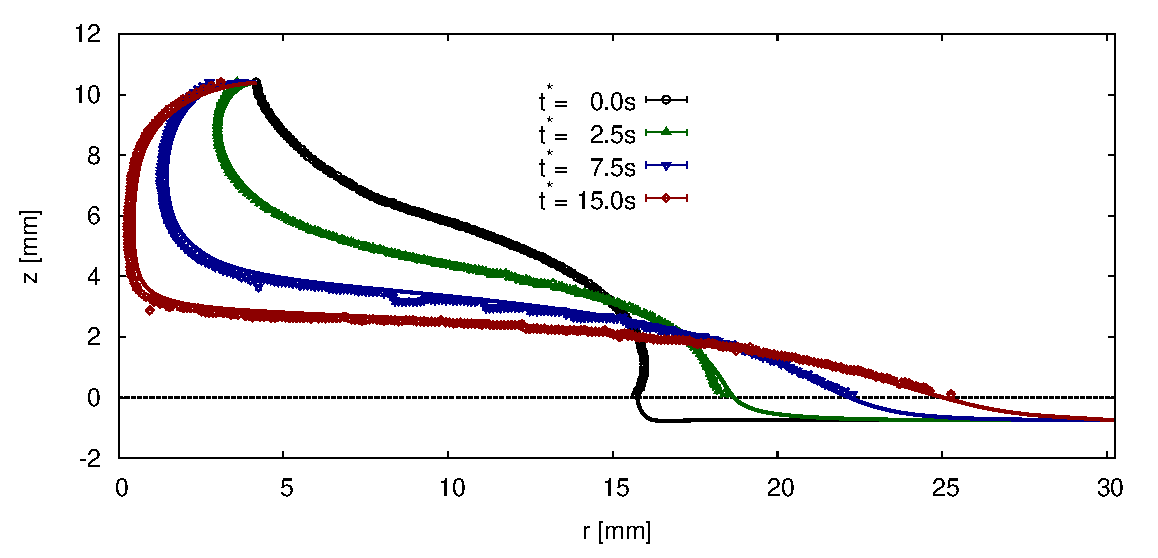
\includegraphics[width=0.9\textwidth]{figures/glucose_thick_layer_8_fs_dim_gap_0.75mm.eps}
 \rput(-2.0,4.5){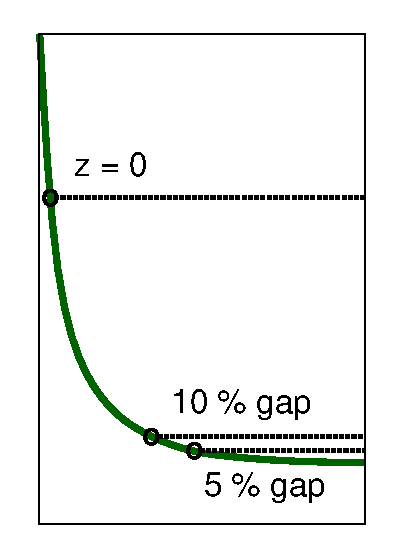
\includegraphics[width=0.19\textwidth]{figures/glucose_thick_layer_8_fs_dim_gap_0.75mm_meas_pt.eps}}
\end{postscript}
\caption{Free surface at different times for a layer thickness of $h^*=1.25$ mm compared against the experiment. Points represent the free surface shape in the experiment; lines represent the computed free surface. Inset shows different measurement points for the drop radius.}
\label{fig:glucose_thick_layer_8_fs_dim_gap_0.75mm}
\end{figure}

The computed shape of the free surface of the spreading drop, $\vect{R}^*_{\sym{fs}}(t)$, at different dimensional times $t^*$ is compared against the experimentally determined shape in figure \ref{fig:glucose_thick_layer_8_fs_dim_gap_0.75mm}, where the error bars represent the pixelation error of the image analysis.
There is excellent agreement between the computations and experiment and the computations provide additional insight into the profile for $z<0$.
As the drop spreads out its height reduces and the fluid thread between the bulk of the drop and the residual fluid in the nozzle outlet narrows.
The radius of this thread decreases, resulting eventually in pinch-off due to the Plateau-Rayleigh instability.
However, the computation was stopped before the pinch-off.
Moreover, there is a significant change of the free surface shape in the region between the drop and the fluid layer.
Initially, the curvature in this region is high, but as the drop spreads the interface is pushed out and the curvature decreases until the free surface forms a wedge which advances.

\begin{figure}[!ht]
\centering
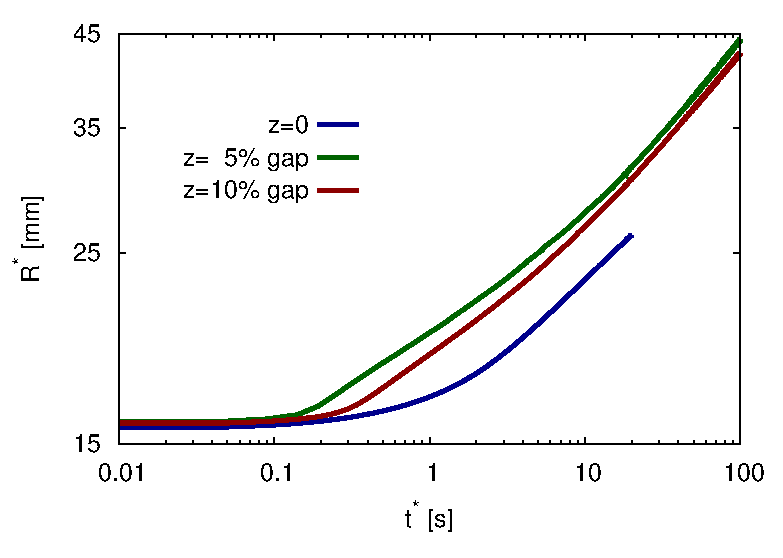
\includegraphics[width=0.6\textwidth]{figures/radius_vs_time_measure_pos_dim.eps}
\caption{Temporal evolution of the drop radius at different measurement points on a log-log scale.}
\label{fig:glucose_thick_layer_8_radius_vs_time_non_dim}
\end{figure}

The evolution of the drop radius is shown in figure \ref{fig:glucose_thick_layer_8_radius_vs_time_non_dim} on a log-log scale at different measurement points.
The radius is determined at the level of the platform edge, as in the experiment, and at the points where the gap is 5\% and 10\% filled (see figure \ref{fig:glucose_thick_layer_8_fs_dim_gap_0.75mm}).
The radius evolution at $z=0$ is not plotted over the entire range, because at larger times the drop height decreases to $H^* < 0$ and hence no radius at $z=0$ can be determined.
Also shown in figure \ref{fig:glucose_thick_layer_8_radius_vs_time_non_dim} is the spreading law of $n$=1/5, which applies to the radius evolution at $z=0$, but for the other two measurement points the spreading law differs.
The drop spreading based on the radius determined at a 5\% and 10\% filled gap, respectively, is similar and the spreading law is identical for $t^*>20$ s.
The spreading based on the radius at $z=0$ is significantly different and does not represent the actual dynamics.

\begin{figure}[!ht]
\centering
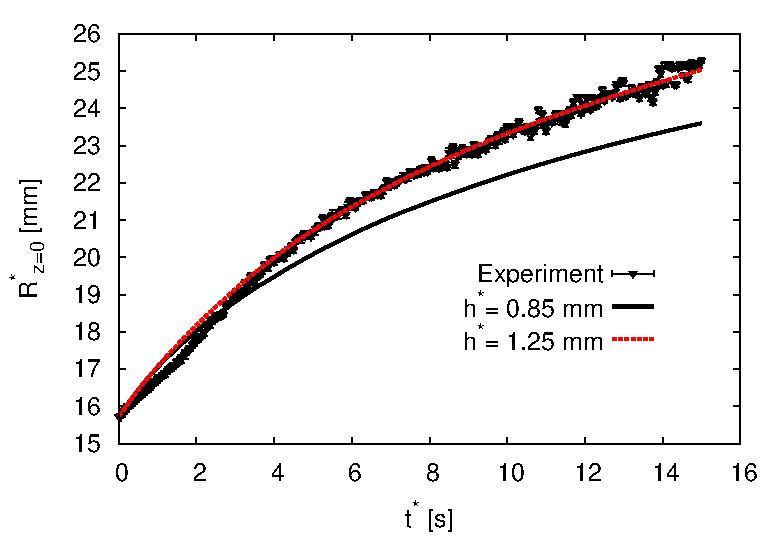
\includegraphics[width=0.6\textwidth]{figures/glucose_thick_layer_8_radius_vs_time_vary_layer.eps}
\caption{Evolution of $R^*_{\sym{contact}}$ over time for varying layer thicknesses $h^*$, compared against the experimentally determined radius.}
\label{fig:glucose_thick_layer_8_radius_vs_time_vary_layer}
\end{figure}

The radius evolution from the experiments at $z=0$ is compared against the computed one in figure \ref{fig:glucose_thick_layer_8_radius_vs_time_vary_layer}, for both the experimentally estimated layer thickness of $h^*=0.85$ mm and the computationally re-constructed layer thickness of $h^*=1.25$ mm, which we determined to fit the experimental radius evolution.
This figure indicates that the layer thickness has strong influence on the drop spreading, which motivated further numerical experiments.

\subsubsection{Influence of layer thickness}

\begin{table}[!ht]
 \centering
 \begin{tabular}{l | >{\centering\arraybackslash}m{3.5cm} | >{\centering\arraybackslash}m{3.5cm} | >{\centering\arraybackslash}m{3.5cm}}
   & \multicolumn{3}{>{\centering\arraybackslash}m{10.5cm}}{$h^*$ in mm} \\ \cline{2-4}
  $t$ & 0.0125 & 1.25 & 12.5 \\ \hline
  0 &
  \begin{postscript}
   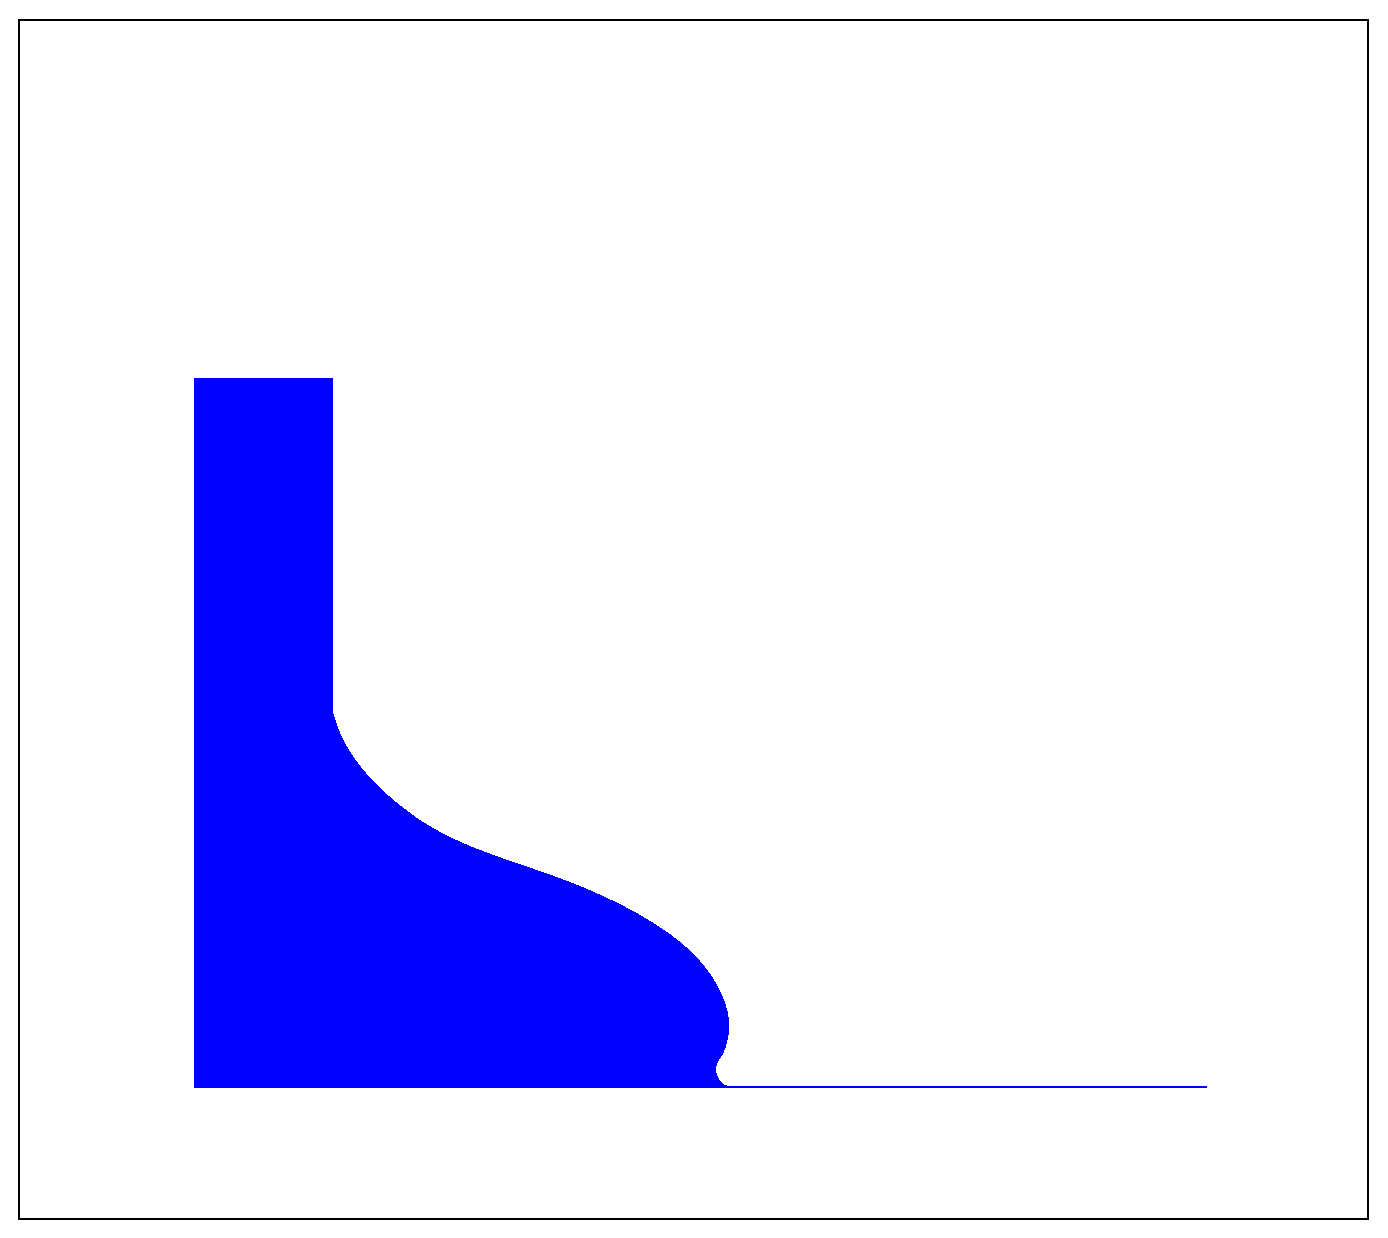
\includegraphics[trim={45px 35px 35px 35px},clip,width=3.2cm]{figures/glucose_layer_0_0125mm_0_t_0.eps}
   \rput(-1.0,1.7){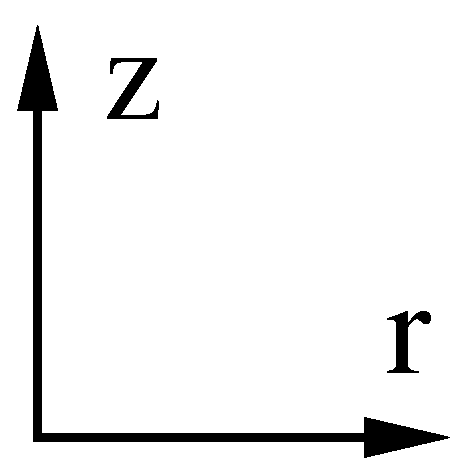
\includegraphics[width=1.25cm]{figures/axisym_coord.eps}}
  \end{postscript}
   & 
  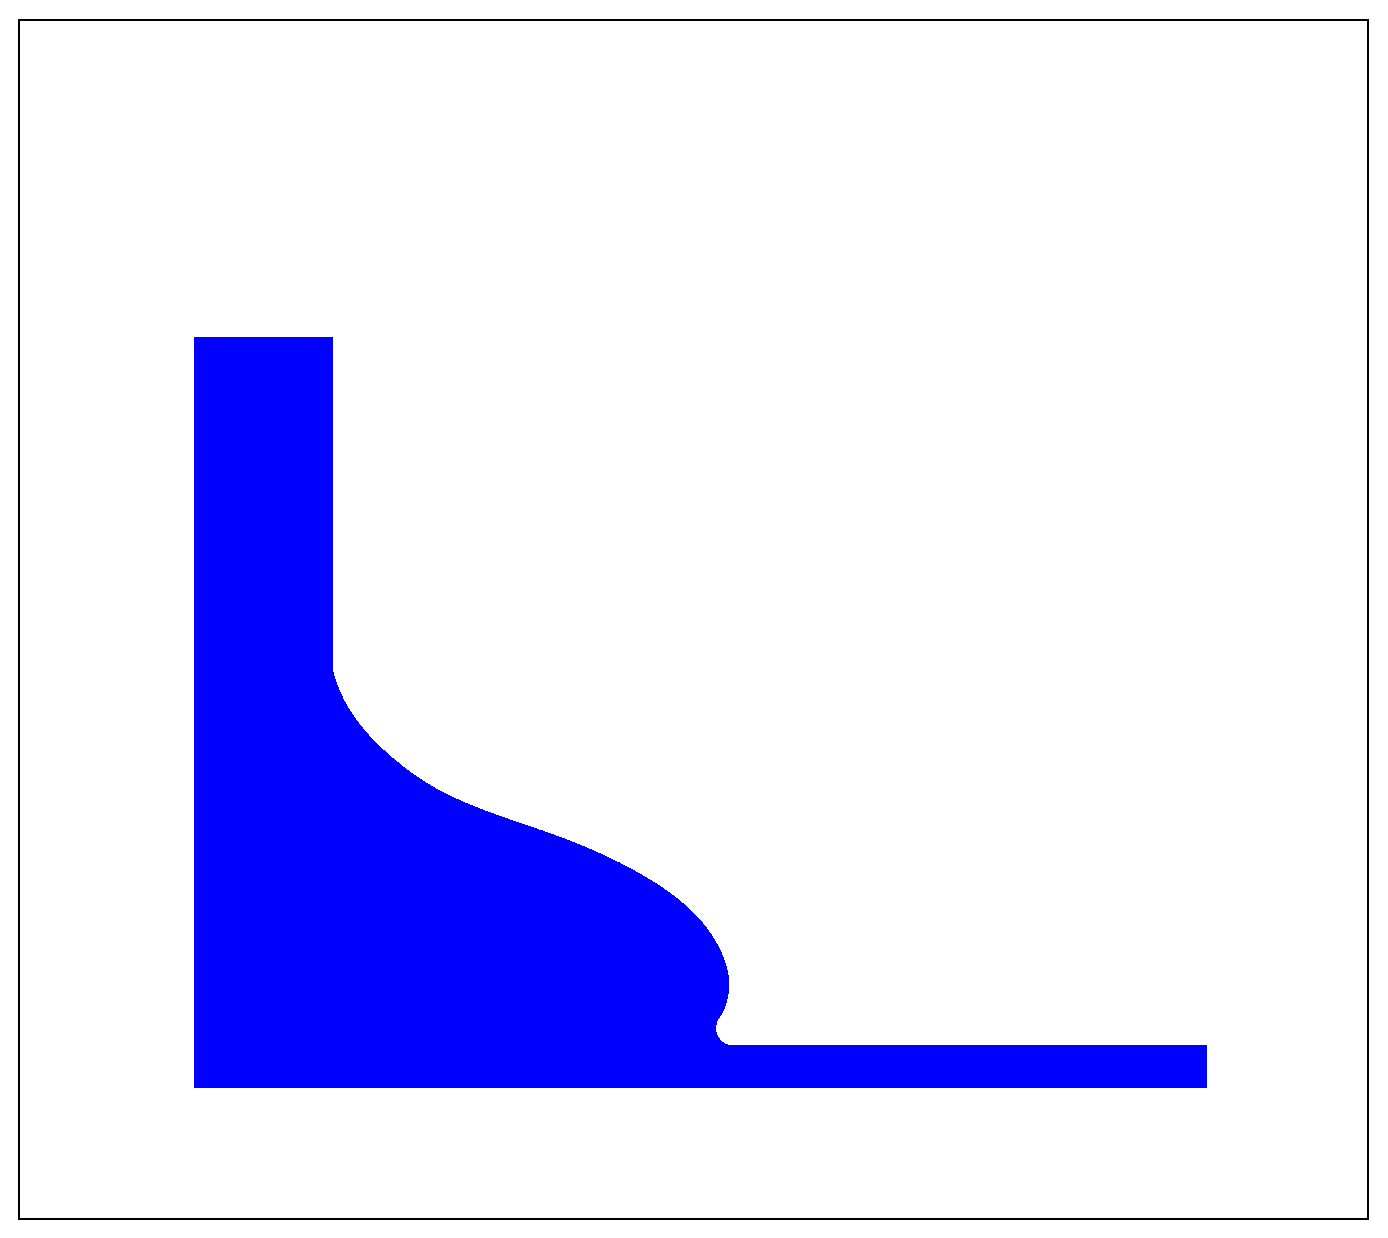
\includegraphics[trim={45px 35px 35px 35px},clip,width=3.2cm]{figures/glucose_layer_1_25mm_0_t_0.eps} & 
  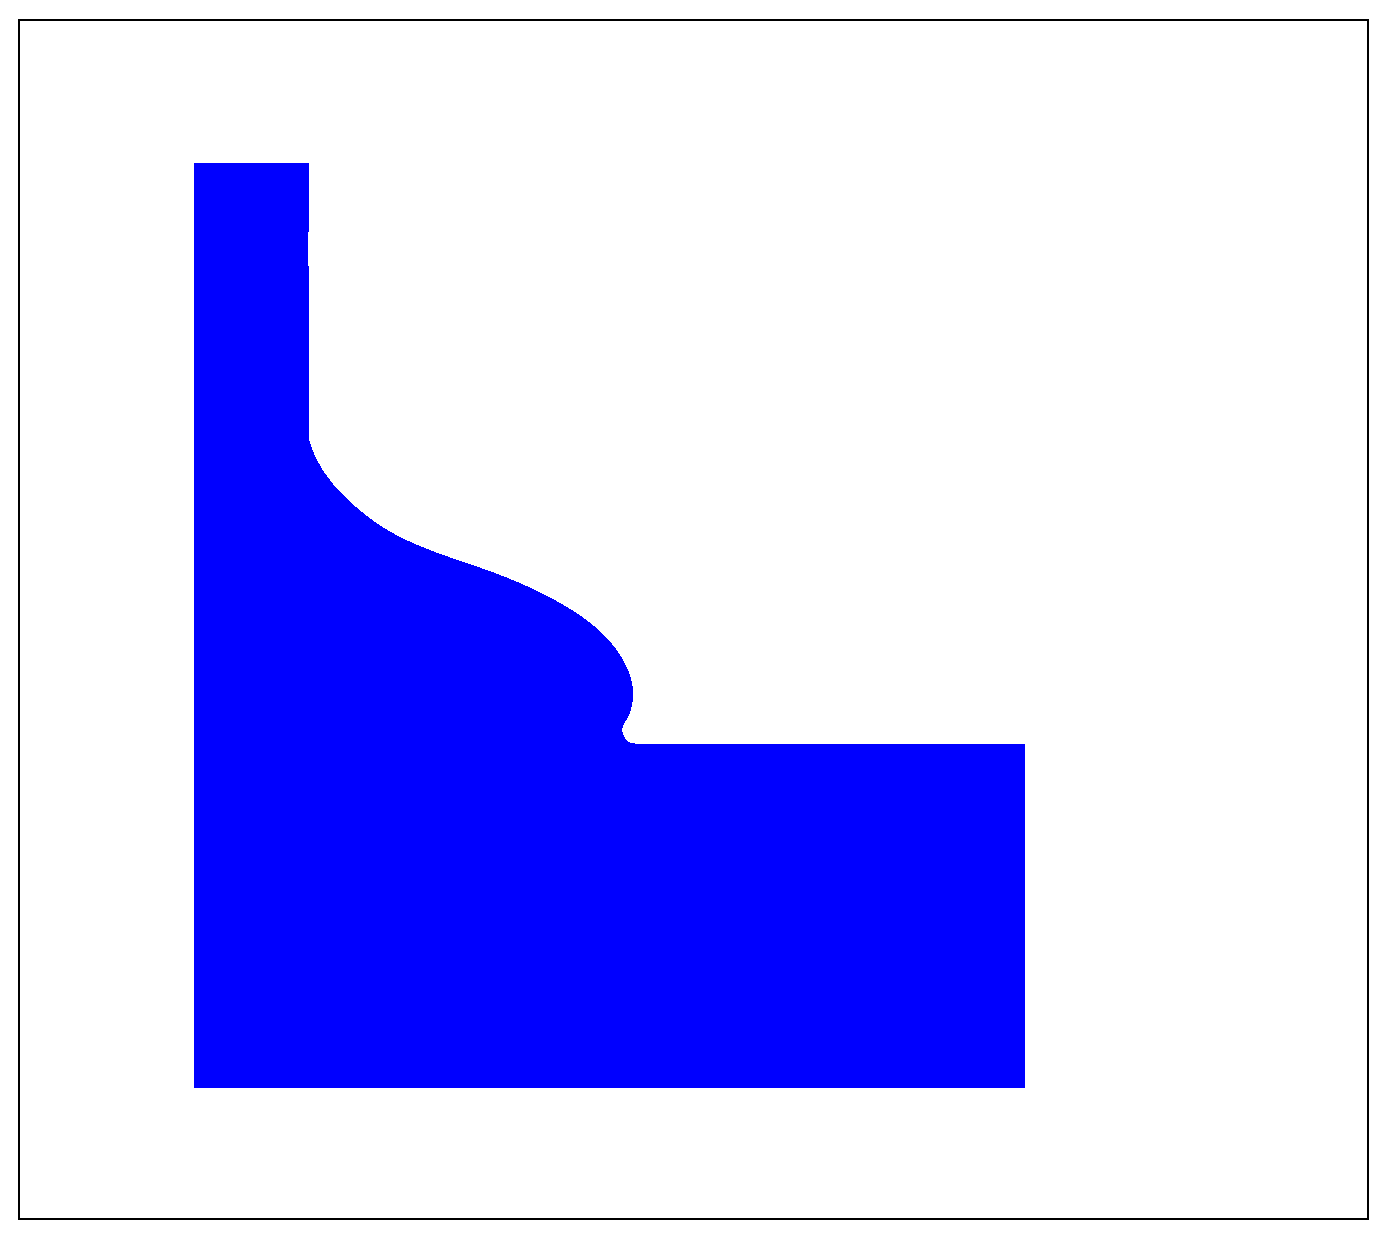
\includegraphics[trim={45px 35px 35px 35px},clip,width=3.2cm]{figures/glucose_layer_12_5mm_0_t_0.eps} \\ \hline
  2 & 
  \begin{postscript}
   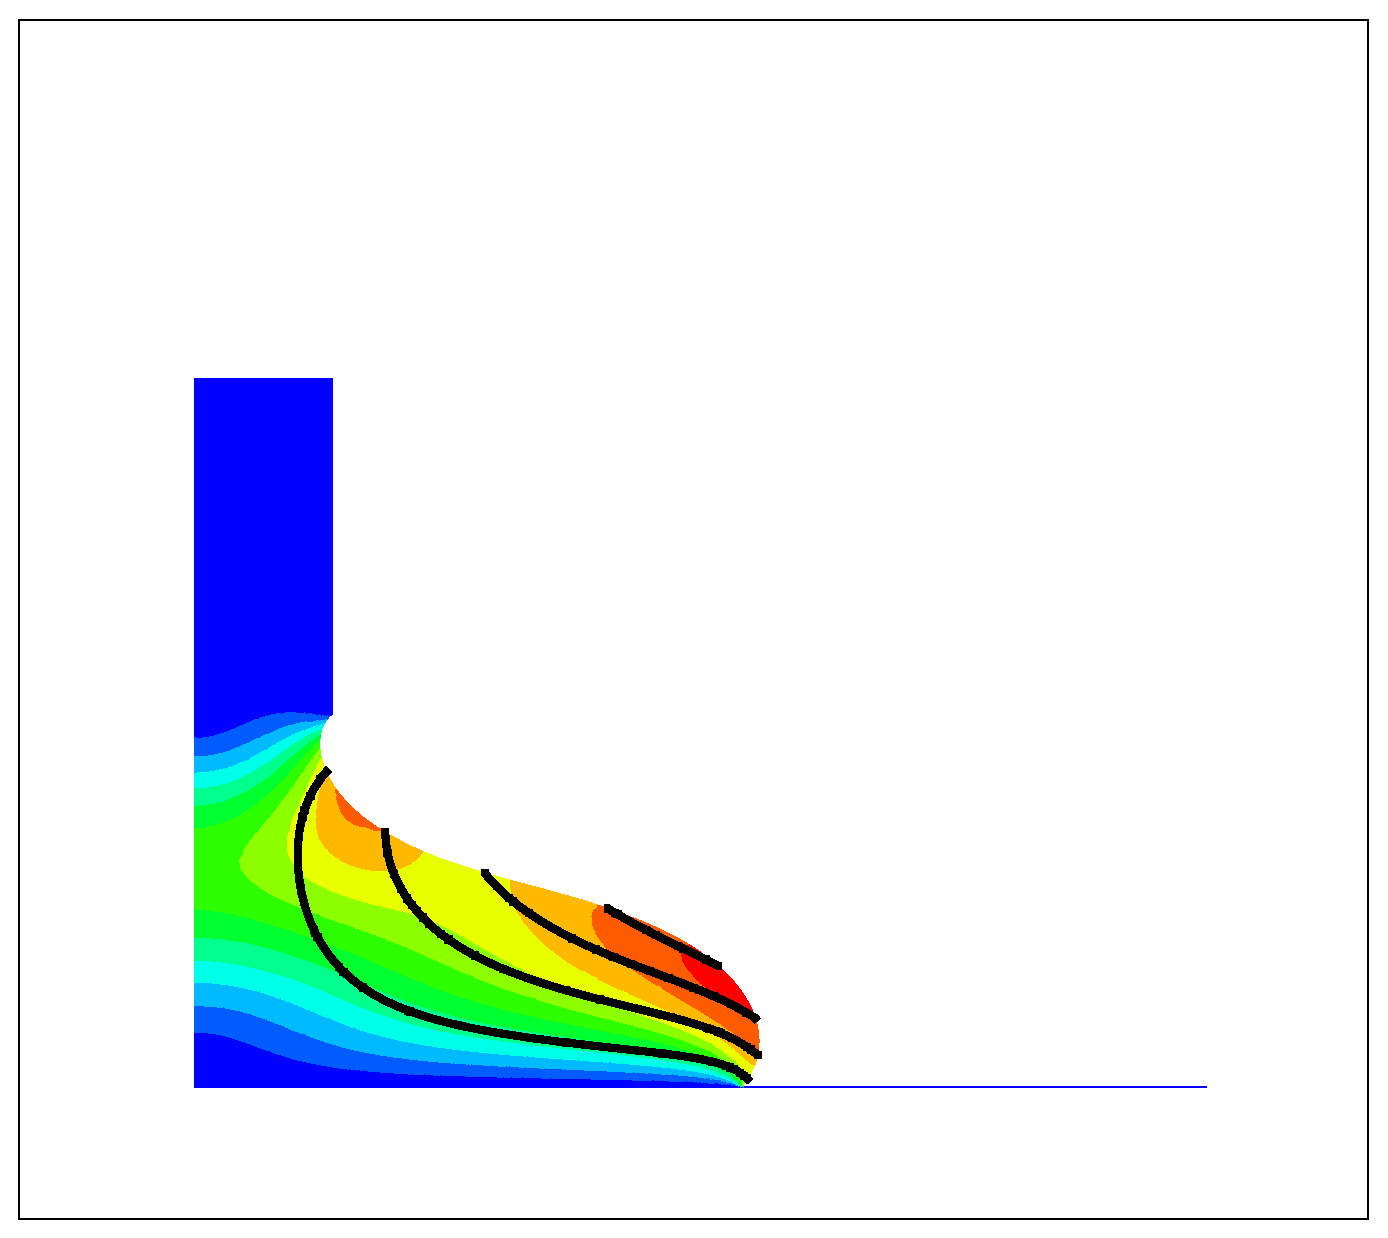
\includegraphics[trim={45px 35px 35px 35px},clip,width=3.2cm]{figures/glucose_layer_0_0125mm_84_t_2.eps}
   \rput(-1.0,1.7){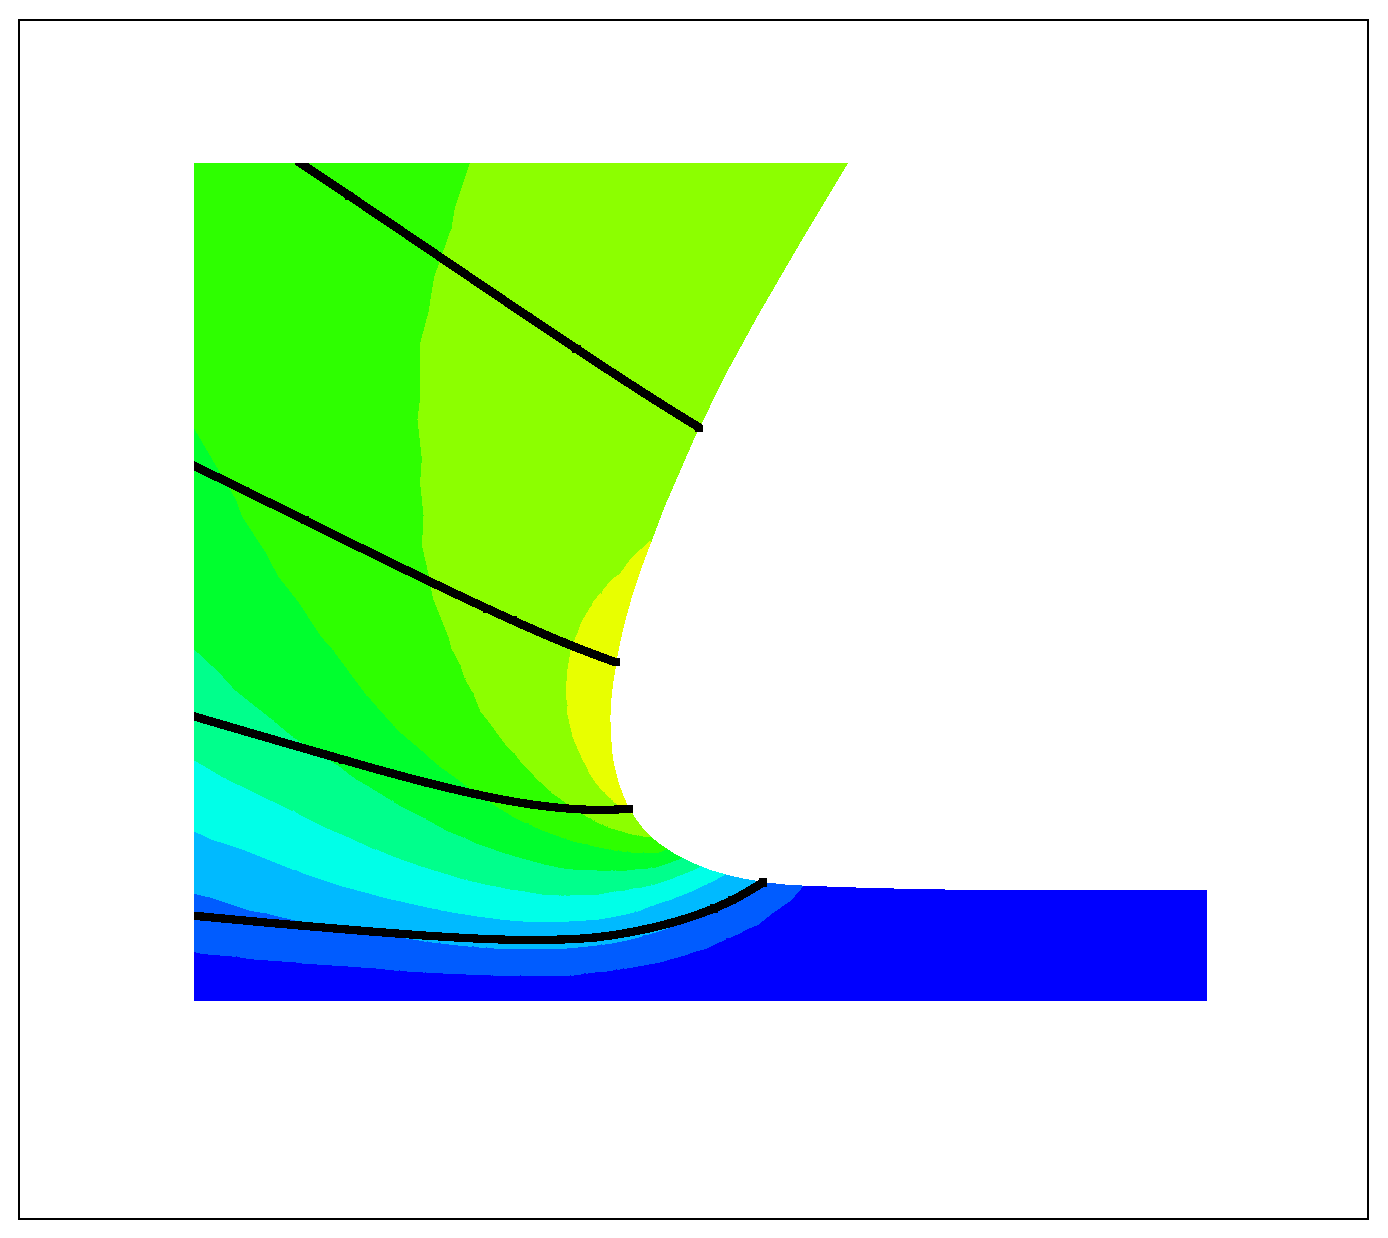
\includegraphics[width=1.75cm]{figures/glucose_layer_0_0125mm_84_t_2_inset2.eps}}
  \end{postscript}
   & 
  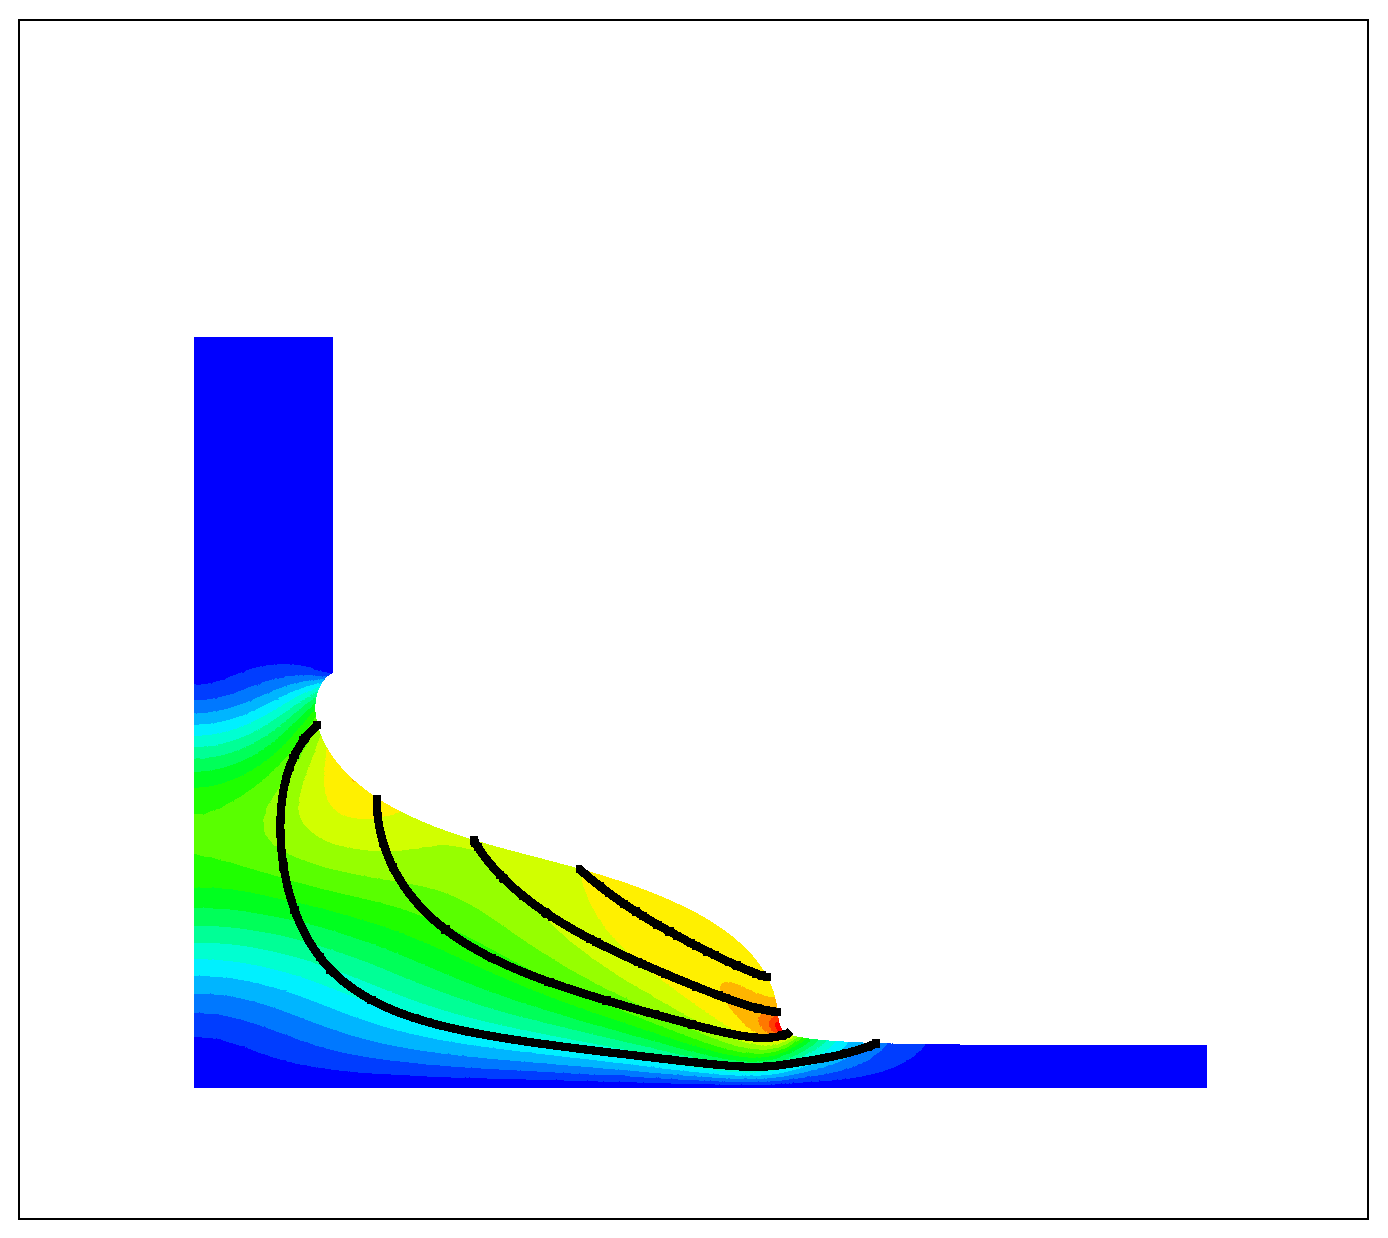
\includegraphics[trim={45px 35px 35px 35px},clip,width=3.2cm]{figures/glucose_layer_1_25mm_28_t_2.eps} & 
  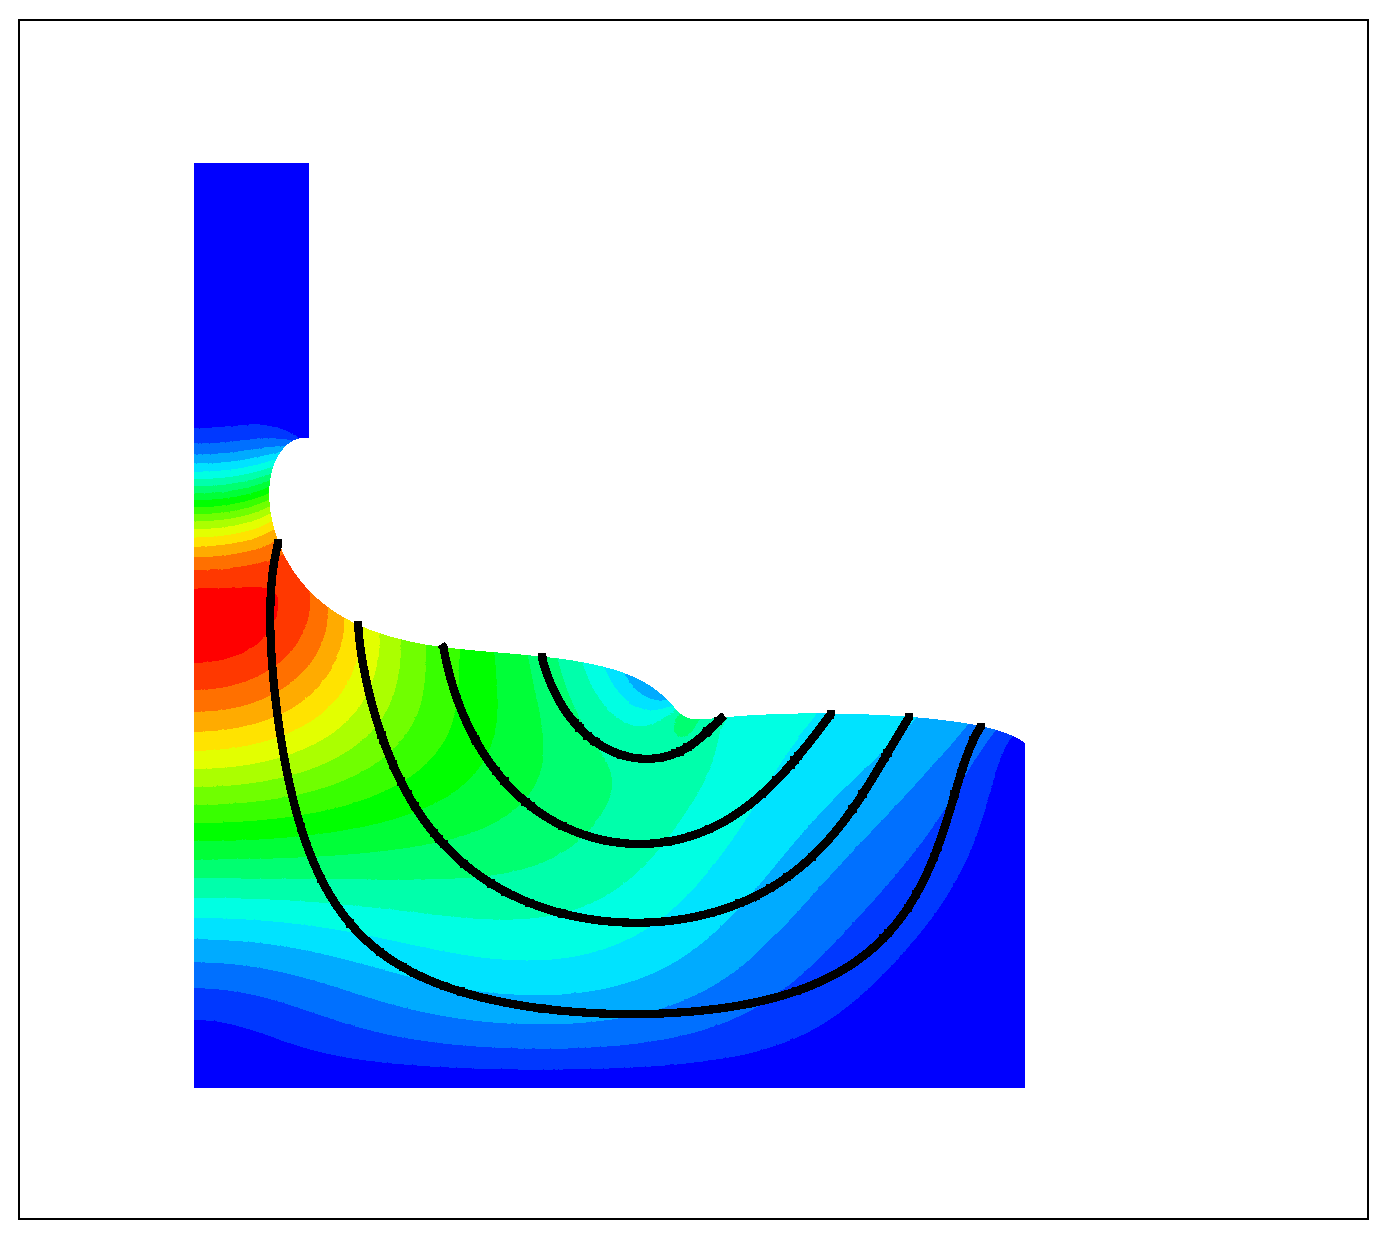
\includegraphics[trim={45px 35px 35px 35px},clip,width=3.2cm]{figures/glucose_layer_12_5mm_32_t_2.eps} \\ \hline
  4 & 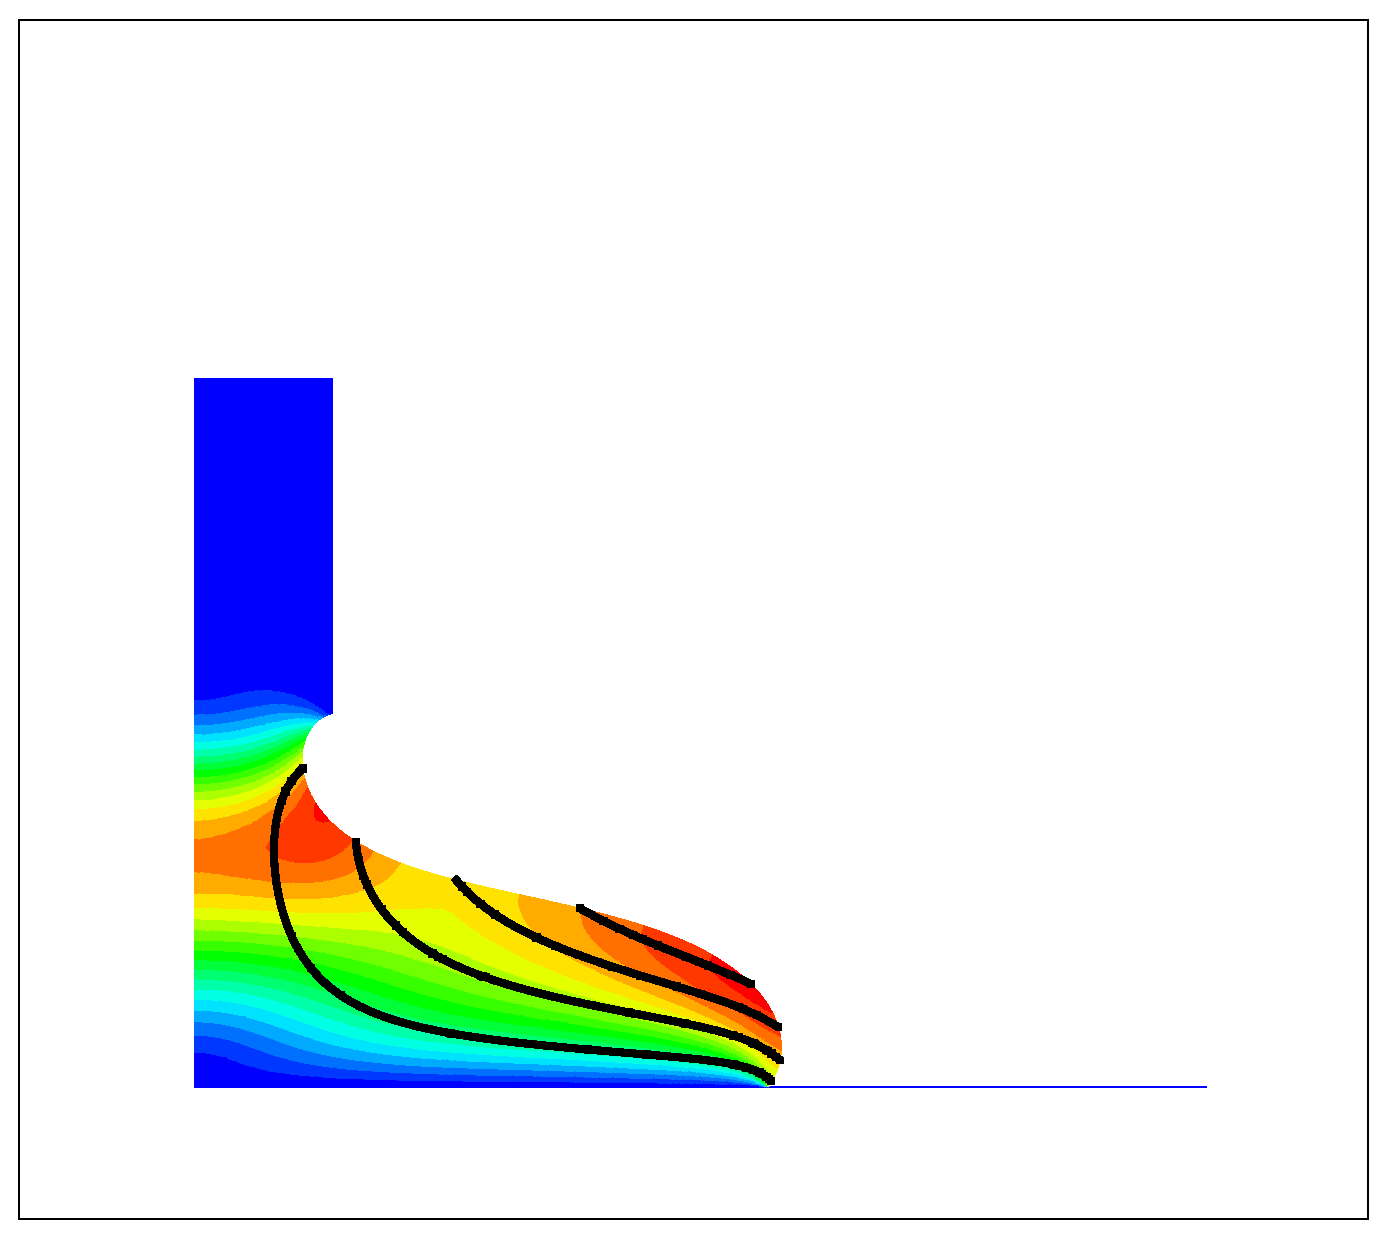
\includegraphics[trim={45px 35px 35px 35px},clip,width=3.2cm]{figures/glucose_layer_0_0125mm_277_t_4.eps} & 
  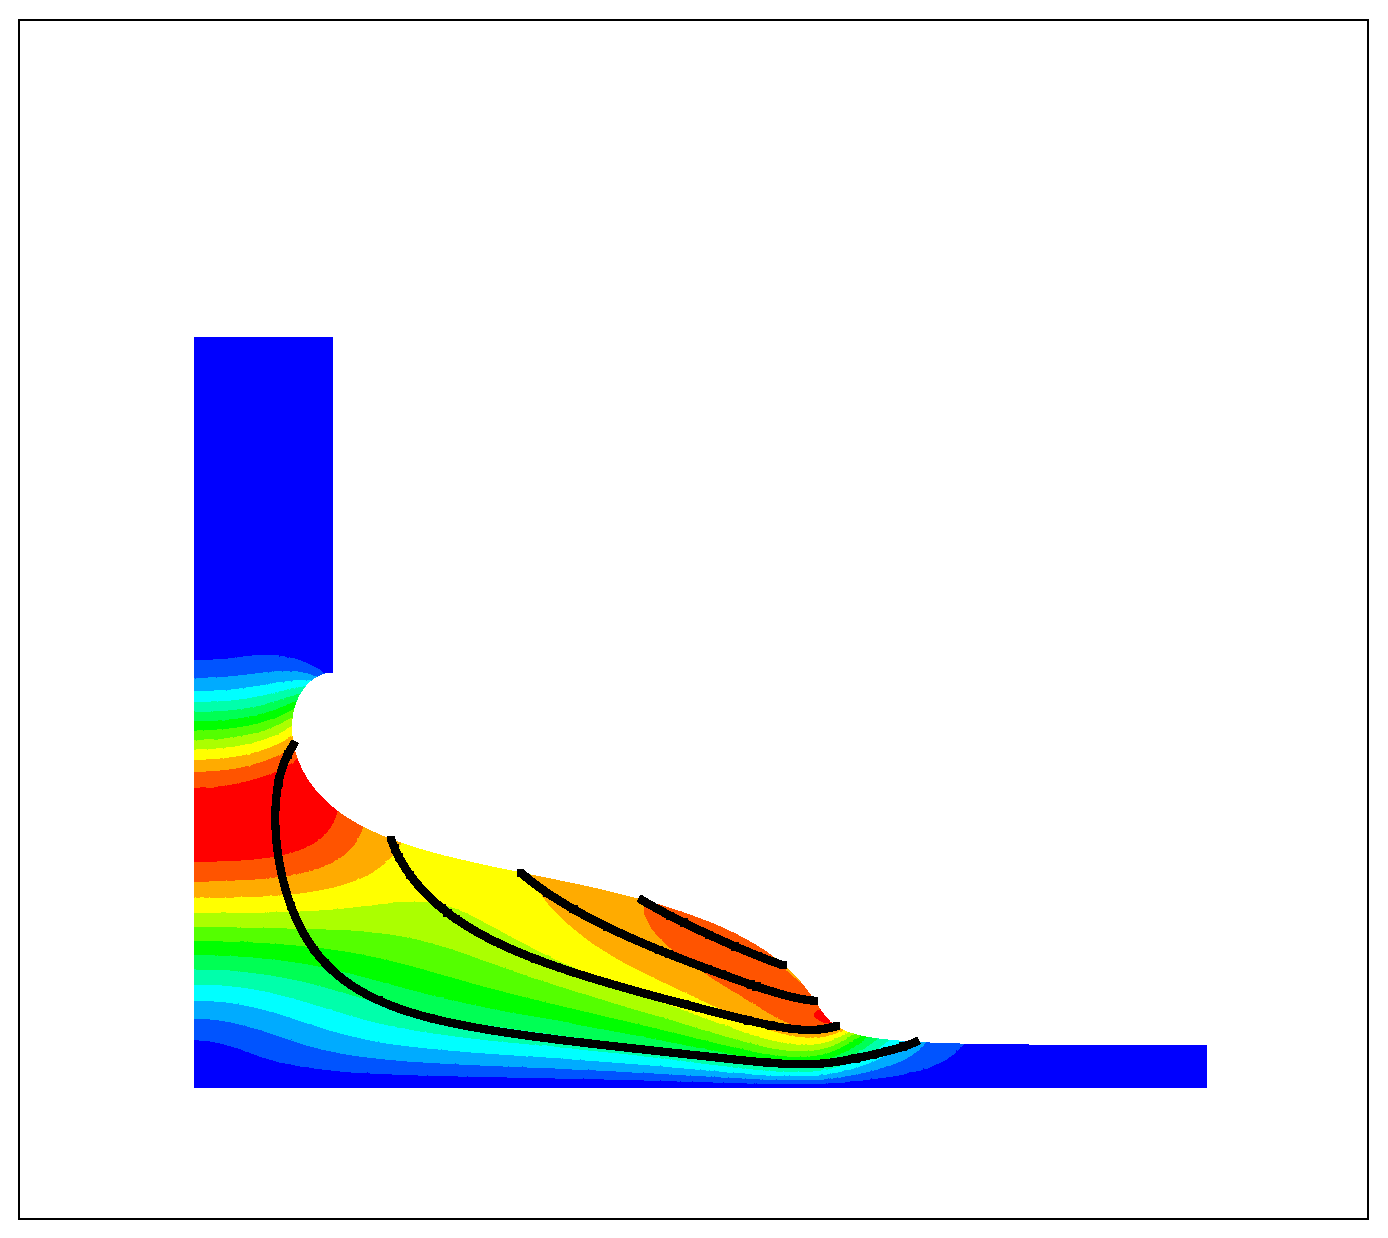
\includegraphics[trim={45px 35px 35px 35px},clip,width=3.2cm]{figures/glucose_layer_1_25mm_57_t_4.eps} & 
  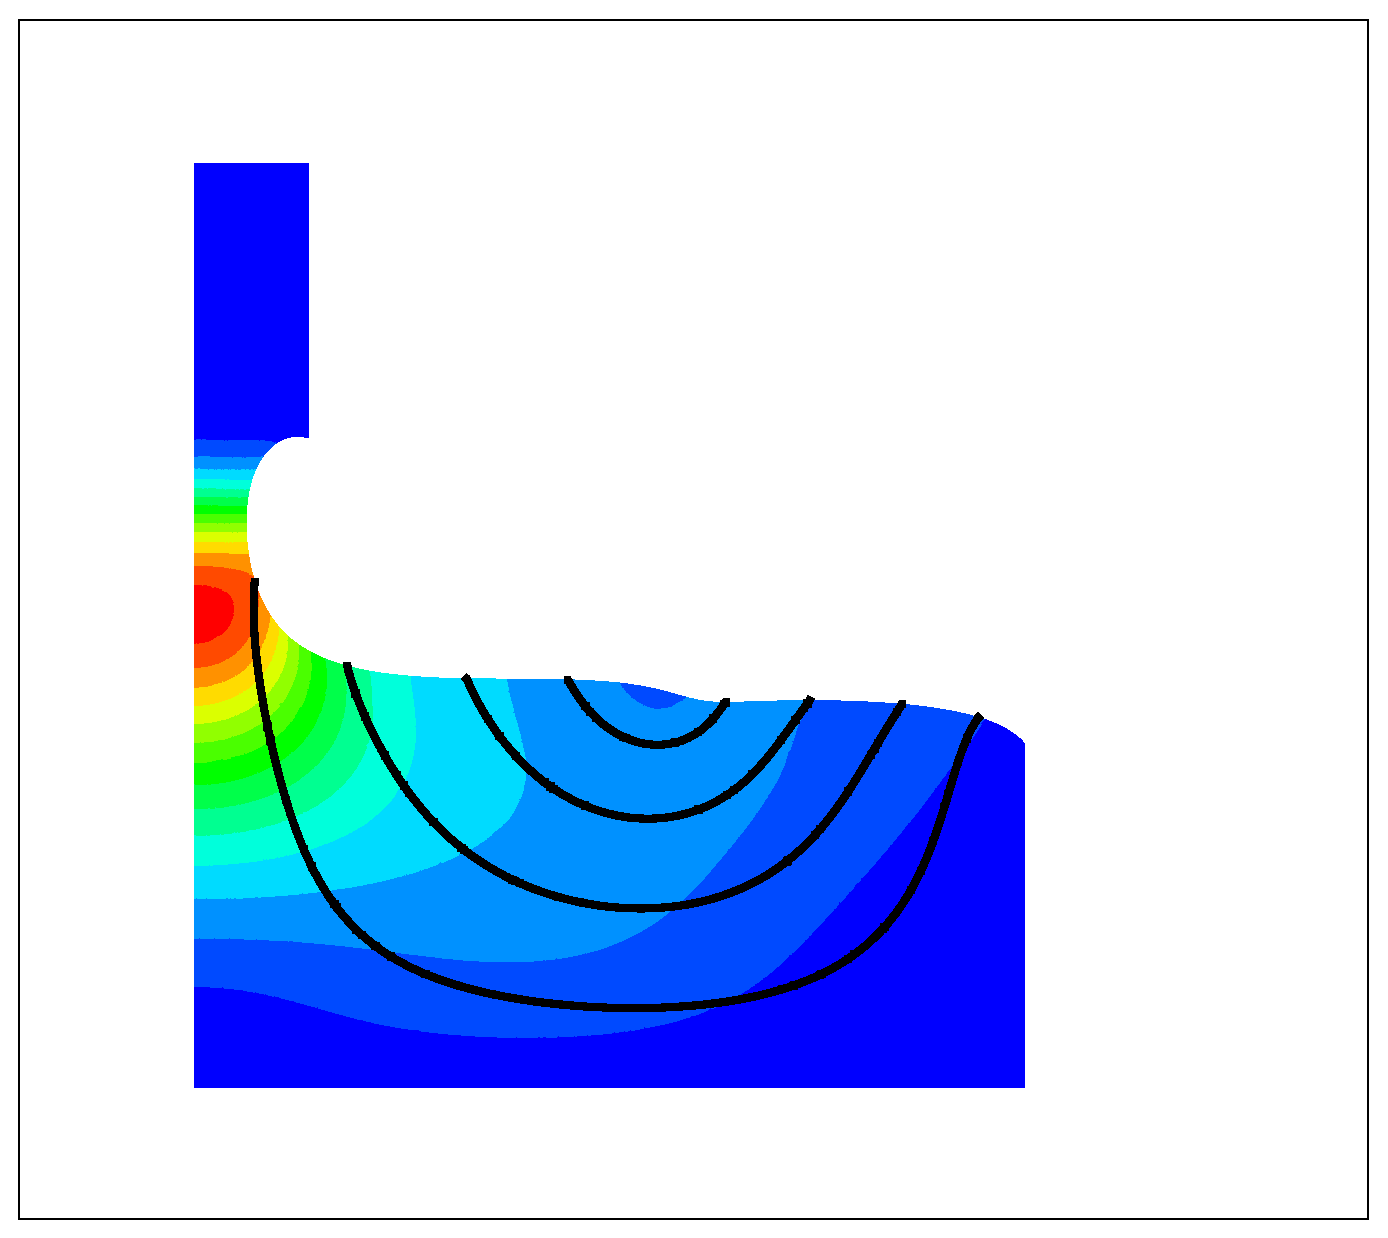
\includegraphics[trim={45px 35px 35px 35px},clip,width=3.2cm]{figures/glucose_layer_12_5mm_60_t_4.eps} \\ \hline
  20 & 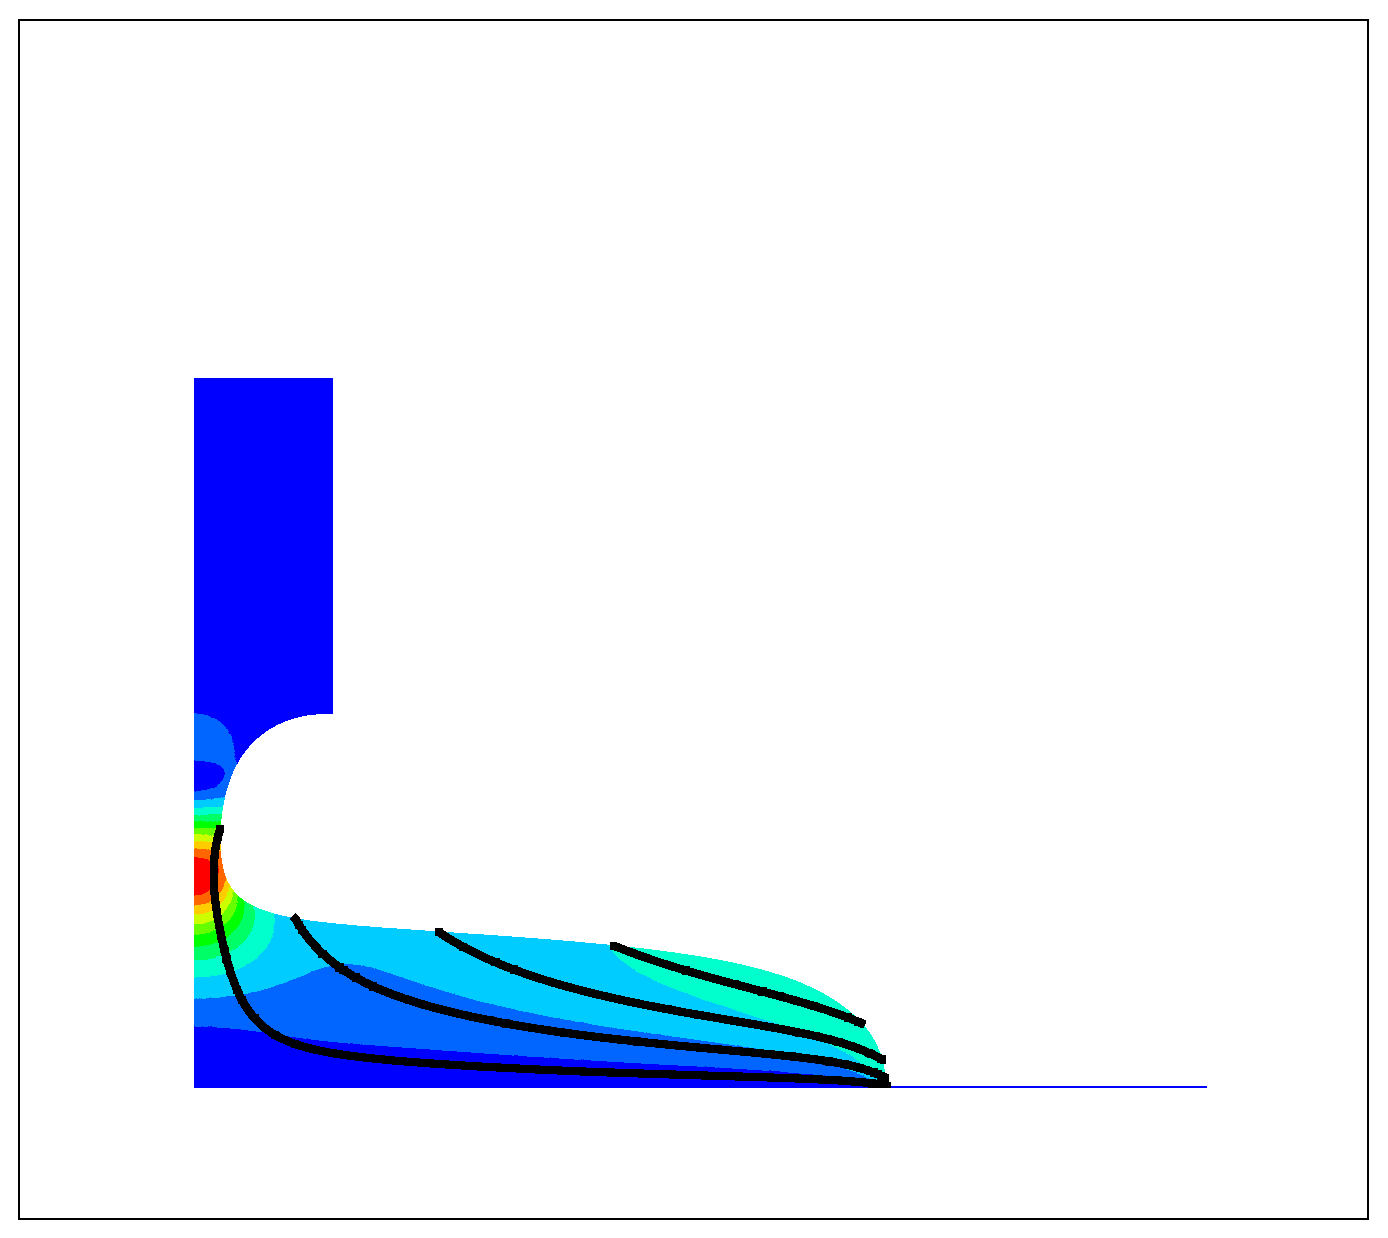
\includegraphics[trim={45px 35px 35px 35px},clip,width=3.2cm]{figures/glucose_layer_0_0125mm_893_t_20.eps} & 
  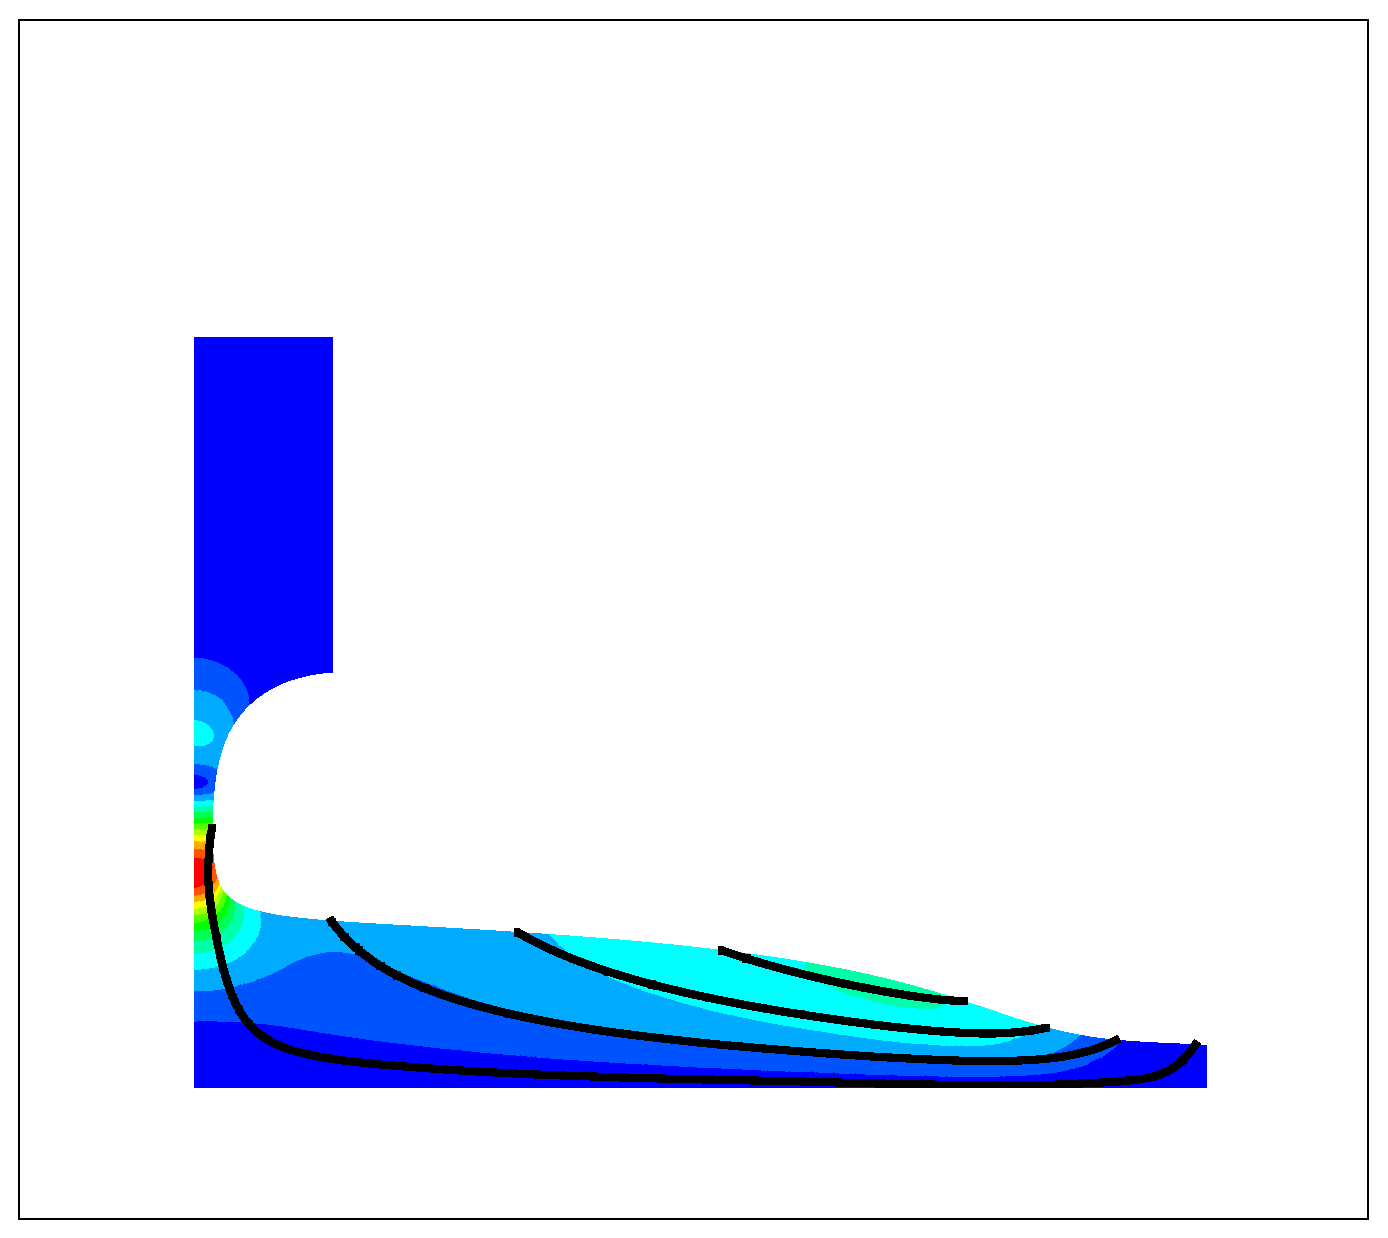
\includegraphics[trim={45px 35px 35px 35px},clip,width=3.2cm]{figures/glucose_layer_1_25mm_281_t_20.eps} & 
  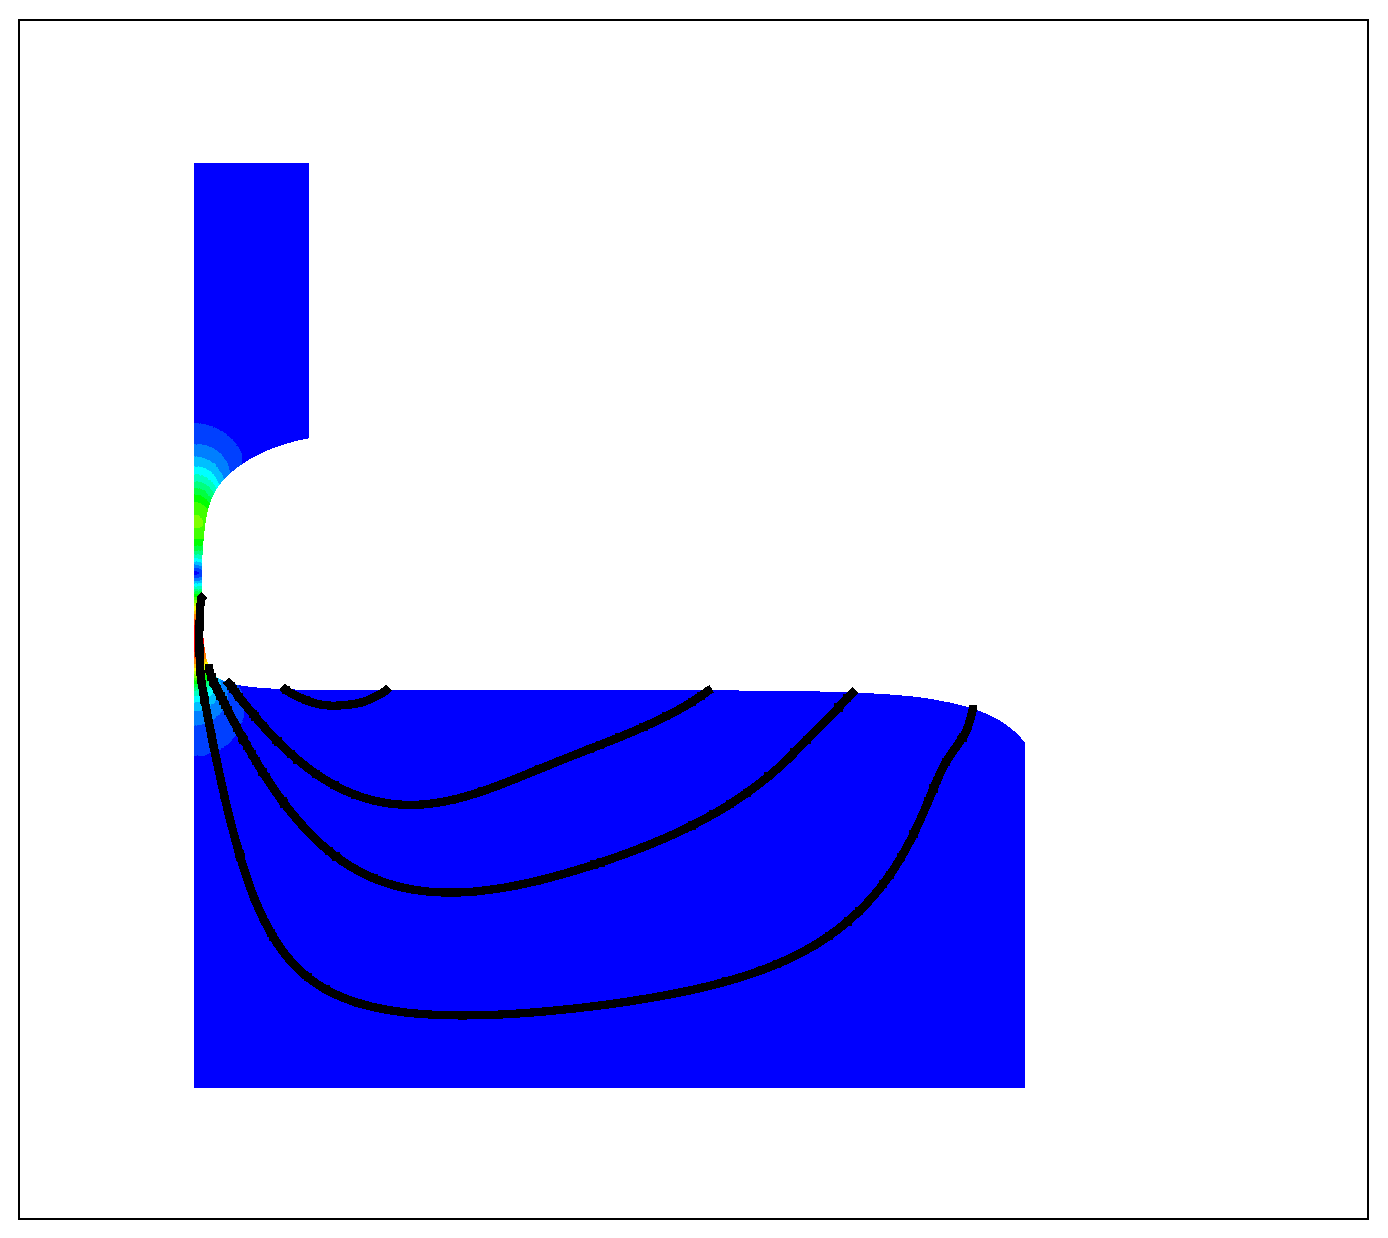
\includegraphics[trim={45px 35px 35px 35px},clip,width=3.2cm]{figures/glucose_layer_12_5mm_285_t_20.eps} \\
 \end{tabular}
 \caption{Illustration of different spreading regimes for different layer thicknesses. The contours represent the magnitude of the velocity $|u|=\sqrt{u_r^2+u_z^2}$ and the streamlines illustrate the velocity field.}
 \label{tab:spreading_regimes}
\end{table}

The same drop spreading on significantly varying layer thicknesses is illustrated in the sequences in table \ref{tab:spreading_regimes}.
The contours show the magnitude of the flow velocity and the black lines are representative stream lines.
The rate of spreading as well as the shape of the drop as it spreads vary significantly depending on the layer thickness.
For a comparatively thick film of $h^*=12.5$ mm the stream lines indicate that the drop sinks in. 
The flow is predominantly in the layer, which at $t=2$ results in a bulge of the free surface ahead of the actual drop contact.
With decreasing layer thickness there is less flow in the layer and the drop is spreading instead of sinking in.
However, the spreading mechanism for a layer thickness of 1.25 mm and 0.0125 mm differs as illustrated in table \ref{tab:spreading_regimes}.
In case of a layer thickness of 1.25 mm the drop spreads by fluid flowing into the layer and pushing the free surface upwards in the contact region, as shown by the stream lines.
This leads to the formation of a wedge, which constantly advances and is sustained by the flow into the layer ahead.
For a layer thickness of one hundreth of this value, the fluid no longer flows ahead into the layer and pushes the interface up.
Instead, the drop spreads through flow into the contact region which pushes the interface radially outward. \\


\begin{figure}[!ht]
\centering
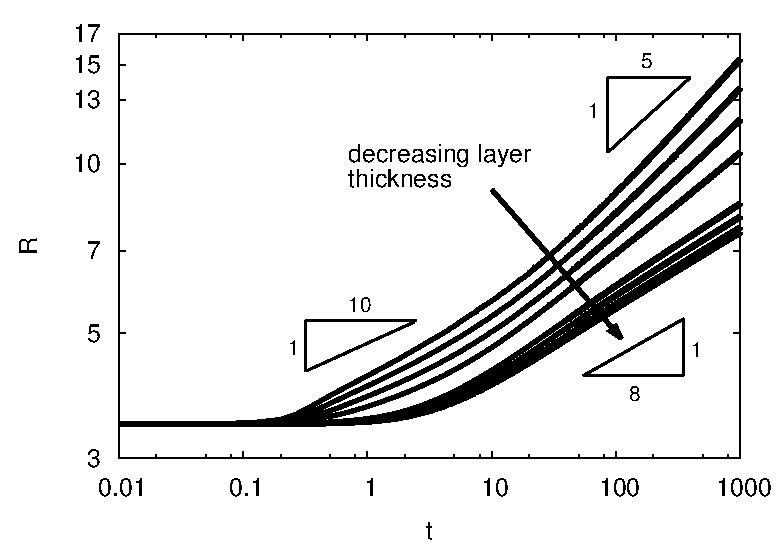
\includegraphics[width=0.6\textwidth]{figures/radius_vs_time_before_and_after_pinch_off.eps}
\caption{Evolution of radius $R$ determined at a 5\% filled gap over time for varying layer thicknesses $h^*=1.25, 1.0, 0.75, 0.5, 0.125, 0.05, 0.0125$ and 0.005 mm.}
\label{fig:radius_vs_time_before_and_after_pinch_off}
\end{figure}

The radius evolution for varying layer thicknesses down to less than one hundreth of the experimental value is shown in figure \ref{fig:radius_vs_time_before_and_after_pinch_off}.
The results indicate a transition from one spreading regime to another as the layer thickness decreases.
In the first regime, covering a layer thickness $h^*$ from 1.25 to 0.5 mm, the onset of spreading is at around $t=0.3$.
This onset is followed by surface tension dominated spreading, indicated by spreading laws of around $R \propto t^{1/10}$.
This spreading mode is followed by viscous dominated spreading with spreading laws of around $R \propto t^{1/5}$.
The duration of the initial surface tension spreading reduces with layer thickness and eventually vanishes for $h^*=0.125$ mm.
In the second regime, covering a layer thickness $h^*$ from 0.125 to 0.005 mm, the onset of spreading is at around $t=3.0$ and hence noticably delayed compared to the first regime.
Also, spreading laws in this regime close to $R \propto t^{1/8}$ indicate that the entire spreading following onset in the second regime is dominated by gravity \cite{cazabat1986dynamics}. \\


In the simulations the liquid thread between the drop and the nozzle is getting thinner, and this geometric restriction limits the extent of the computational results.
In order to cover the temporal range in figure \ref{fig:radius_vs_time_before_and_after_pinch_off} we manually cut this thread and restarted the simulations.
This step can be performed because Re $\ll$ 1 and inertial effects are negligible.

\begin{figure}[!ht]
\centering
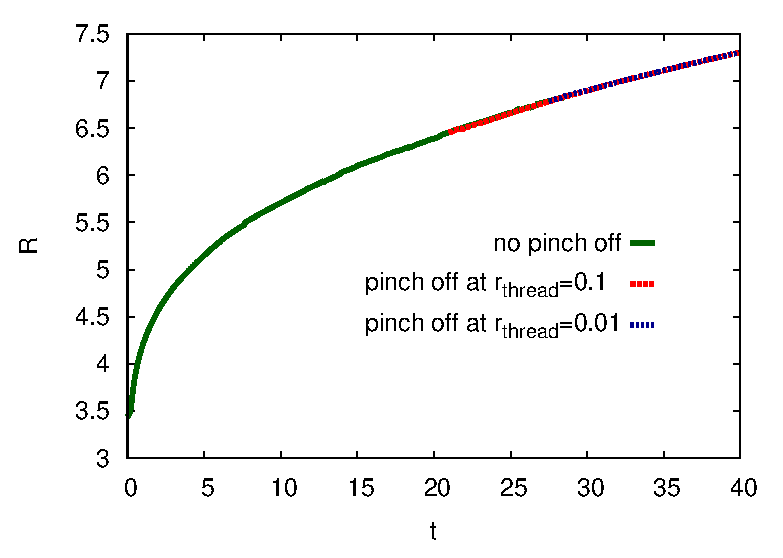
\includegraphics[width=0.6\textwidth]{figures/radius_vs_time_influence_pinch_off.eps}
\caption{Influence of manual pinch off for $h^*=1.25$ mm.}
\label{fig:radius_vs_time_influence_pinch_off}
\end{figure}

To assess the influence of when we disconnect the drop from the nozzle we performed simulations where we cut the thread once its radius reached a value of $r_{\sym{thread}}=0.1$ and 0.01, respectively.
The results are shown in figure \ref{fig:radius_vs_time_influence_pinch_off}, where the radius evolution for the two cases is compared againt the results without pinch off.
There is excellent agreement in all cases, so therefore we arbitrarily chose to disconnect at a thread radius of 0.1 and continue the simulations. \\

\begin{figure}[!ht]
\centering
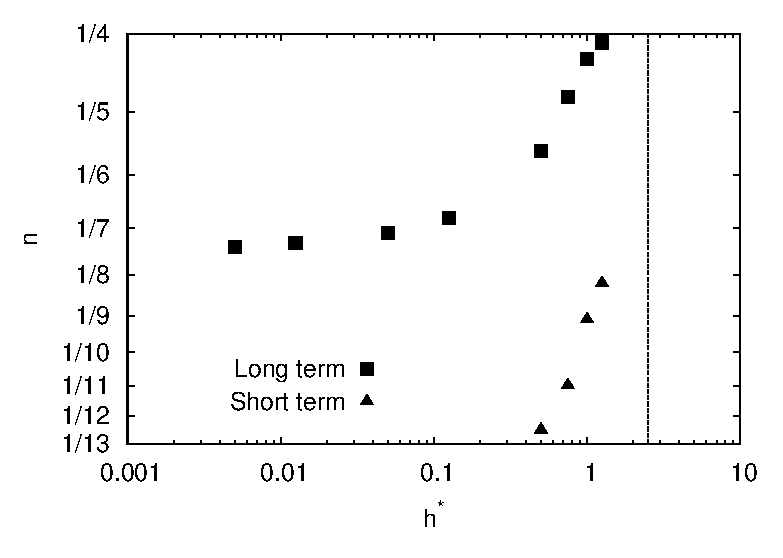
\includegraphics[width=0.6\textwidth]{figures/scaling_vs_layer_inc_short_time.eps}
\caption{Spreading exponent $n$ as function of layer thickness $h^*$ on a log-log scale for both the short term and long term behaviour.}
\label{fig:scaling_vs_layer}
\end{figure}

From figure \ref{fig:radius_vs_time_before_and_after_pinch_off} we extracted radius scaling laws for both the short term and long term behaviour.
The different spreading exponents are shown in figure \ref{fig:scaling_vs_layer} as function of the layer thickness.
Only for layer thicknesses of $h^*=1.25$ to 0.5 mm we were able to extract a distinct short term scaling, as discussed previously.
The dashed line indicates a layer thickness of 2.5 mm at which the drop begins to sink into the layer, similarly to the behaviour observed for $h^*=12.5$ mm in table \ref{tab:spreading_regimes}.
The spreading exponents for the long term behaviour in figure \ref{fig:scaling_vs_layer} confirm the existence of two distinct spreading regimes depending on the layer thickness.
Moreover, they suggest a smooth transition between these two regimes.
The short term, surface tension driven spreading evolves with layer thickness similarly to the long term behaviour. \\


\begin{table}[!ht]
 \centering
 \begin{tabular}{>{\centering\arraybackslash}m{3.5cm}  >{\centering\arraybackslash}m{3.5cm}  >{\centering\arraybackslash}m{3.5cm}}
  \multicolumn{3}{>{\centering\arraybackslash}m{10.5cm}}{$h^*$ in mm} \\
  0.005 & 0.125 & 1.25 \\
   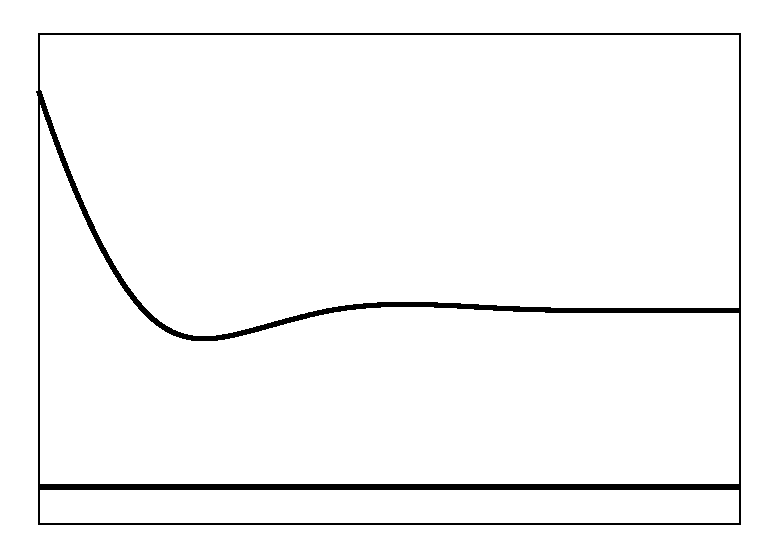
\includegraphics[width=3.2cm]{figures/glucose_layer_0.005mm_free_surface_t_500.eps} & 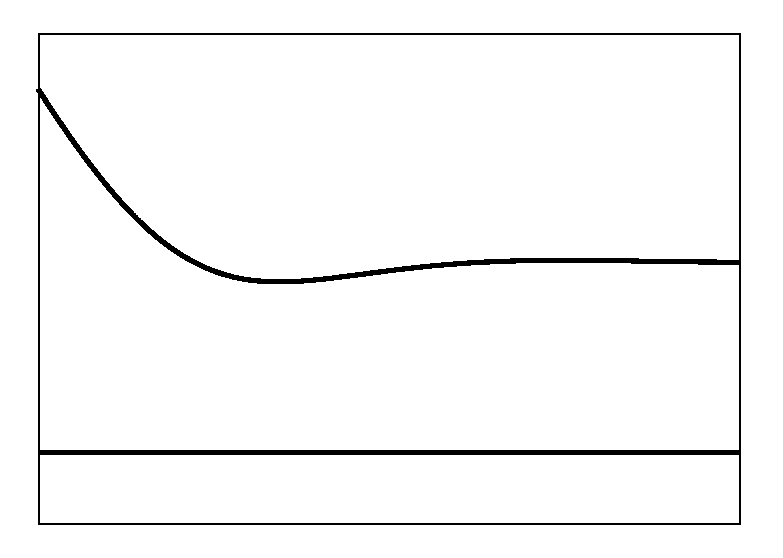
\includegraphics[width=3.2cm]{figures/glucose_layer_0.125mm_free_surface_t_500.eps} & 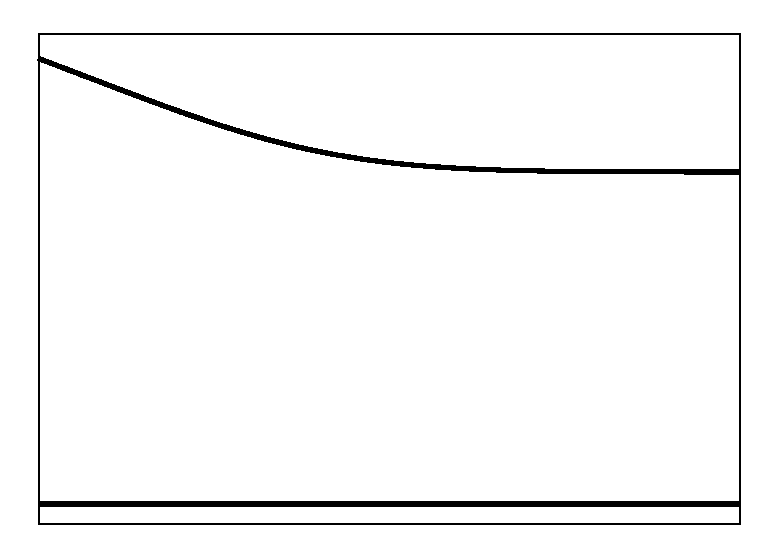
\includegraphics[width=3.2cm]{figures/glucose_layer_1.25mm_free_surface_t_500.eps} \\
 \end{tabular}
 \caption{Shape of the propagating front for selected layer thicknesses.}
 \label{tab:front_shape}
\end{table}

Typical shapes of the spreading front in an established steady state propagation, at $t=500$, are shown in table \ref{tab:front_shape}.
For sufficiently thick layers, in this case $h^*=1.25$ mm, there is a smooth transition from the layer to the drop.
As the layer gets thinner the Landau-Levich meniscus \cite{maleki2011landau} begins to form and the thinner the layer the more pronounced it becomes.
However, a direct comparison to Landau and Levich's theory is not possible, because it is derived for a plate that is withdrawn from a fluid bath.
Their controlling parameter was the speed of the plate, equivalent to our spreading velocity here, and their measured quantity was the residual fluid layer on the plate.
However, in our setup we impose the thickness of the layer instead of treating it as an unknown, and hence Landau and Levich's scaling cannot be applied.


\section{Discussion}

Key findings

\begin{itemize}
 \item spreading on layer viscously dominated, spreading on solid surface tension dominated
 \item spreading on layer, exponent dependent on layer thickness
 \item distinct regimes with or without Landau-Levich meniscus
\end{itemize}


% If in two-column mode, this environment will change to single-column format so that long equations can be displayed. 
% Use only when necessary.
%\begin{widetext}
%$$\mbox{put long equation here}$$
%\end{widetext}

% Figures should be put into the text as floats. 
% Use the graphics or graphicx packages (distributed with LaTeX2e).
% See the LaTeX Graphics Companion by Michel Goosens, Sebastian Rahtz, and Frank Mittelbach for examples. 
%
% Here is an example of the general form of a figure:
% Fill in the caption in the braces of the \caption{} command. 
% Put the label that you will use with \ref{} command in the braces of the \label{} command.
%
% \begin{figure}
% \includegraphics{}%
% \caption{\label{}}%
% \end{figure}

% Tables may be be put in the text as floats.
% Here is an example of the general form of a table:
% Fill in the caption in the braces of the \caption{} command. Put the label
% that you will use with \ref{} command in the braces of the \label{} command.
% Insert the column specifiers (l, r, c, d, etc.) in the empty braces of the
% \begin{tabular}{} command.
%
% \begin{table}
% \caption{\label{} }
% \begin{tabular}{}
% \end{tabular}
% \end{table}

% If you have acknowledgments, this puts in the proper section head.
%\begin{acknowledgments}
% Put your acknowledgments here.
%\end{acknowledgments}

% Create the reference section using BibTeX:
\bibliography{glucose_references}

\end{document}
%
% ****** End of file aiptemplate.tex ******
